The demonstration is organized around the two user-facing clients. The mobile application supports routine market exploration and individual decision support, while Stockrium Lab moves longer-running operations and information-dense result inspection to a larger web workspace. The interfaces are complementary entry points to the same backend services rather than separate analytical systems.

\section{Authentication and Account Management Demo}
\label{sec:demo-authentication-account}

Figure~\ref{fig:stockrium-captures1} demonstrates the authentication entry point, personal watchlist, and profile interface used to manage account-related preferences.

\begin{figure}[H]
    \centering
    \begin{minipage}[t]{0.32\textwidth}
        \vspace{0pt}
        \centering
        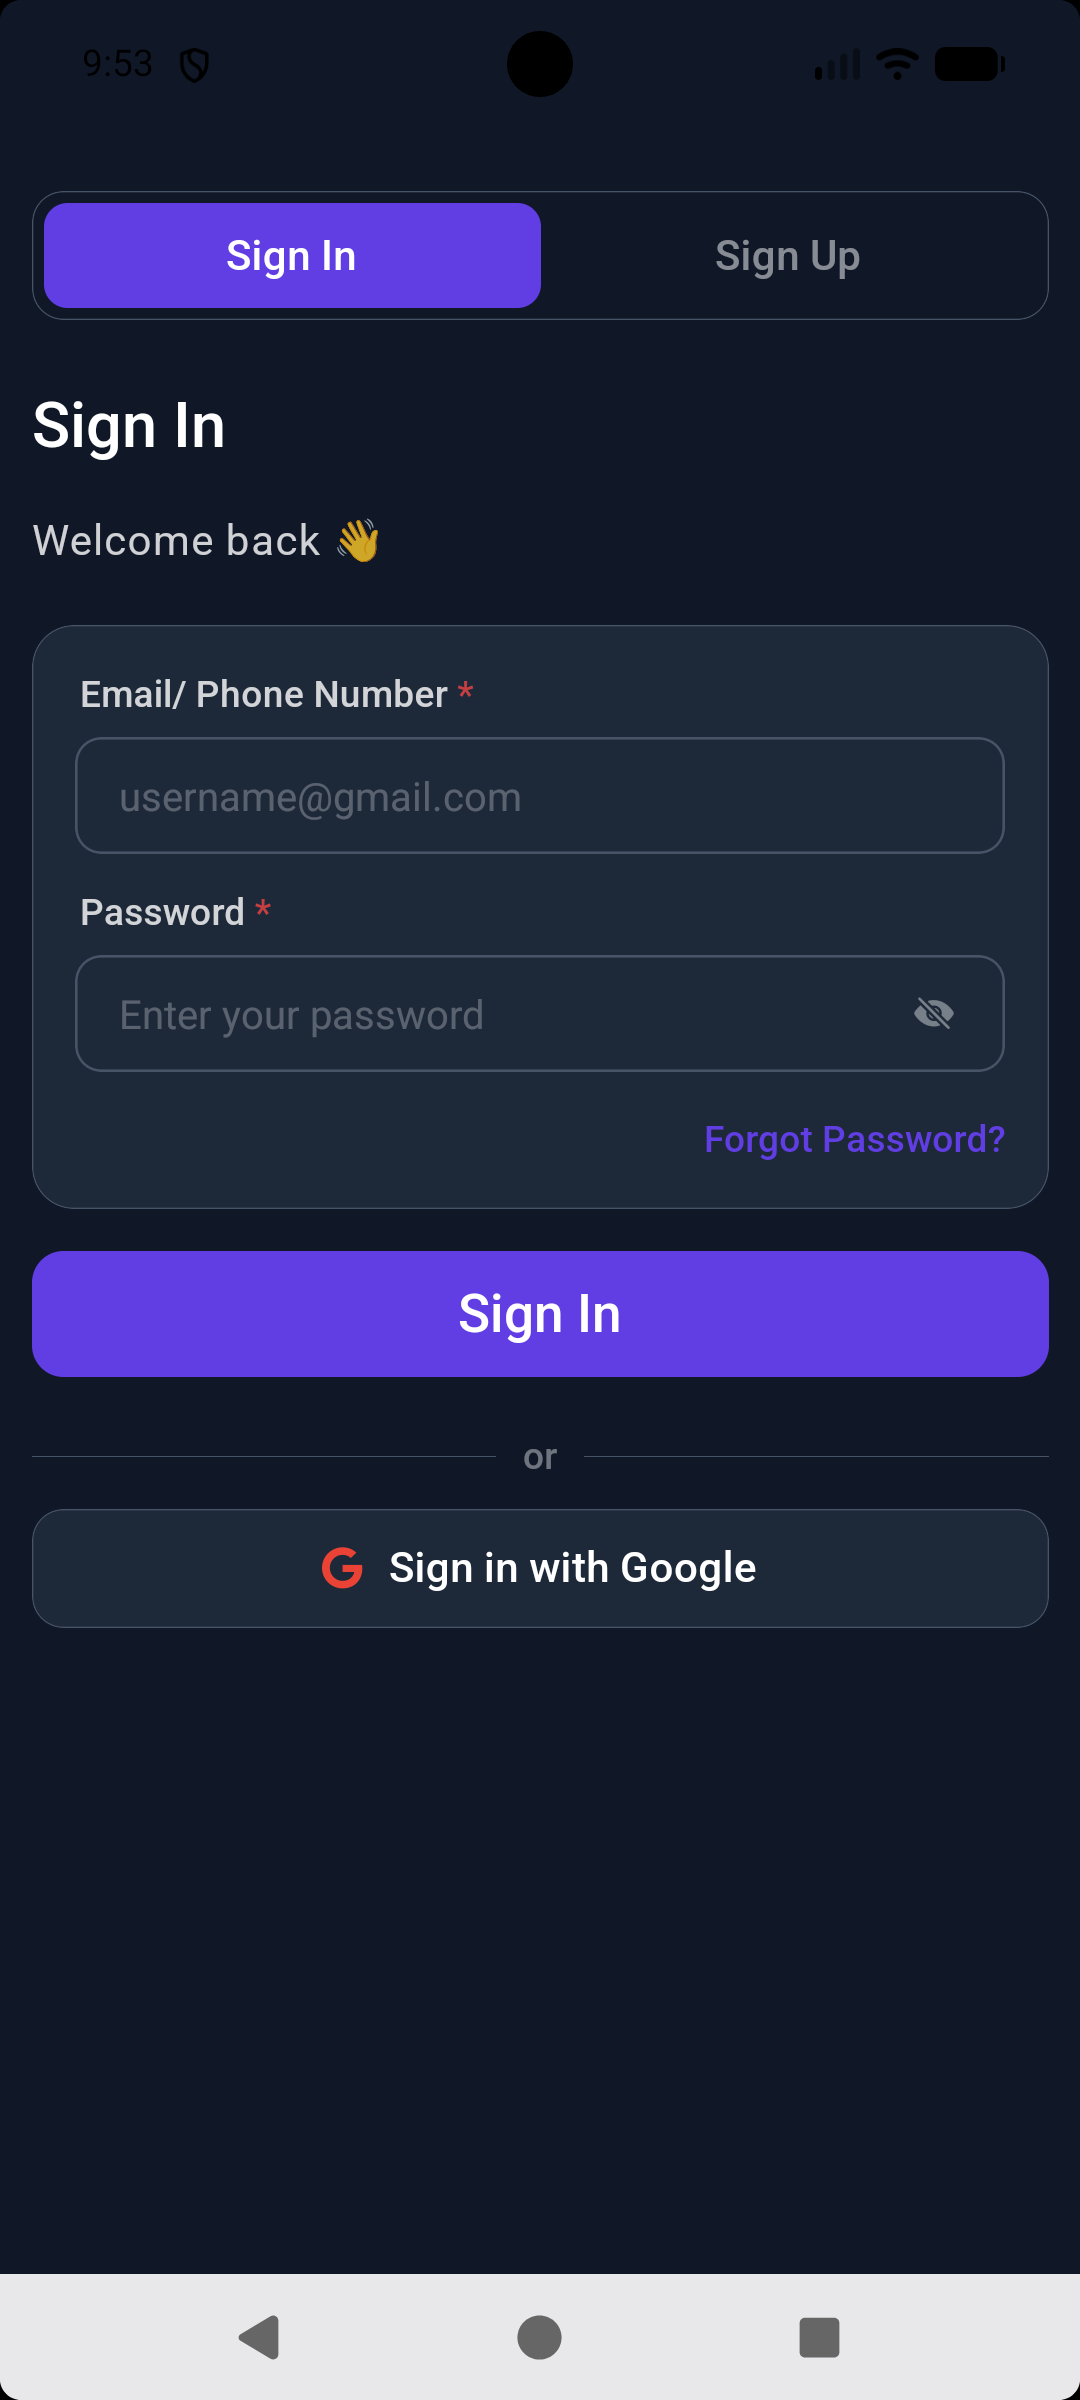
\includegraphics[width=\linewidth]{screenshots/account1.png}\\[2pt]
        \footnotesize (a) Authentication screen
    \end{minipage}%
    \hfill
    \begin{minipage}[t]{0.32\textwidth}
        \vspace{0pt}
        \centering
        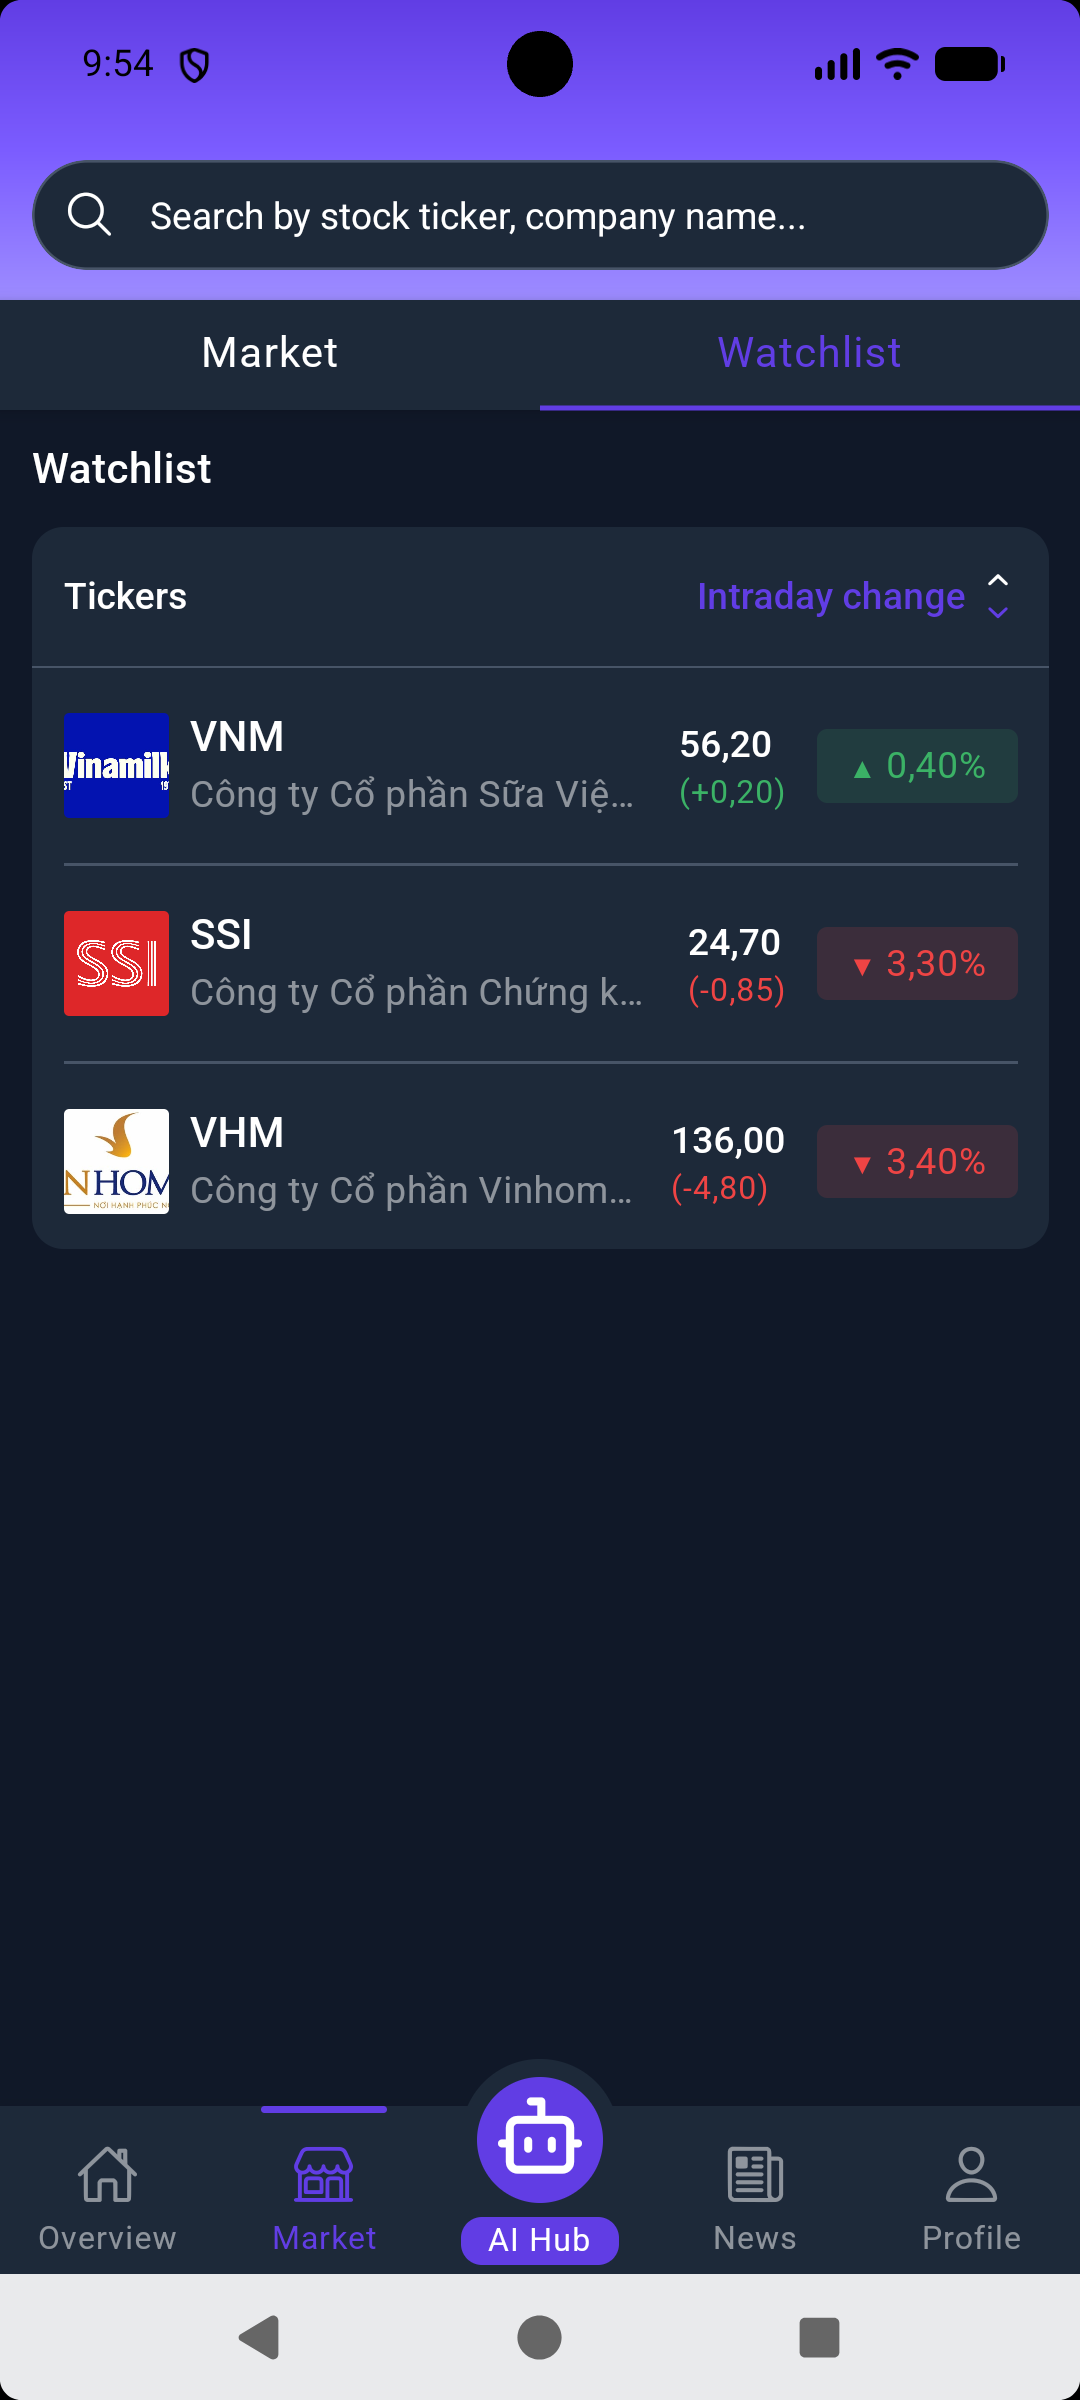
\includegraphics[width=\linewidth]{screenshots/account2.png}\\[2pt]
        \footnotesize (b) Watchlist screen
    \end{minipage}%
    \hfill
    \begin{minipage}[t]{0.32\textwidth}
        \vspace{0pt}
        \centering
        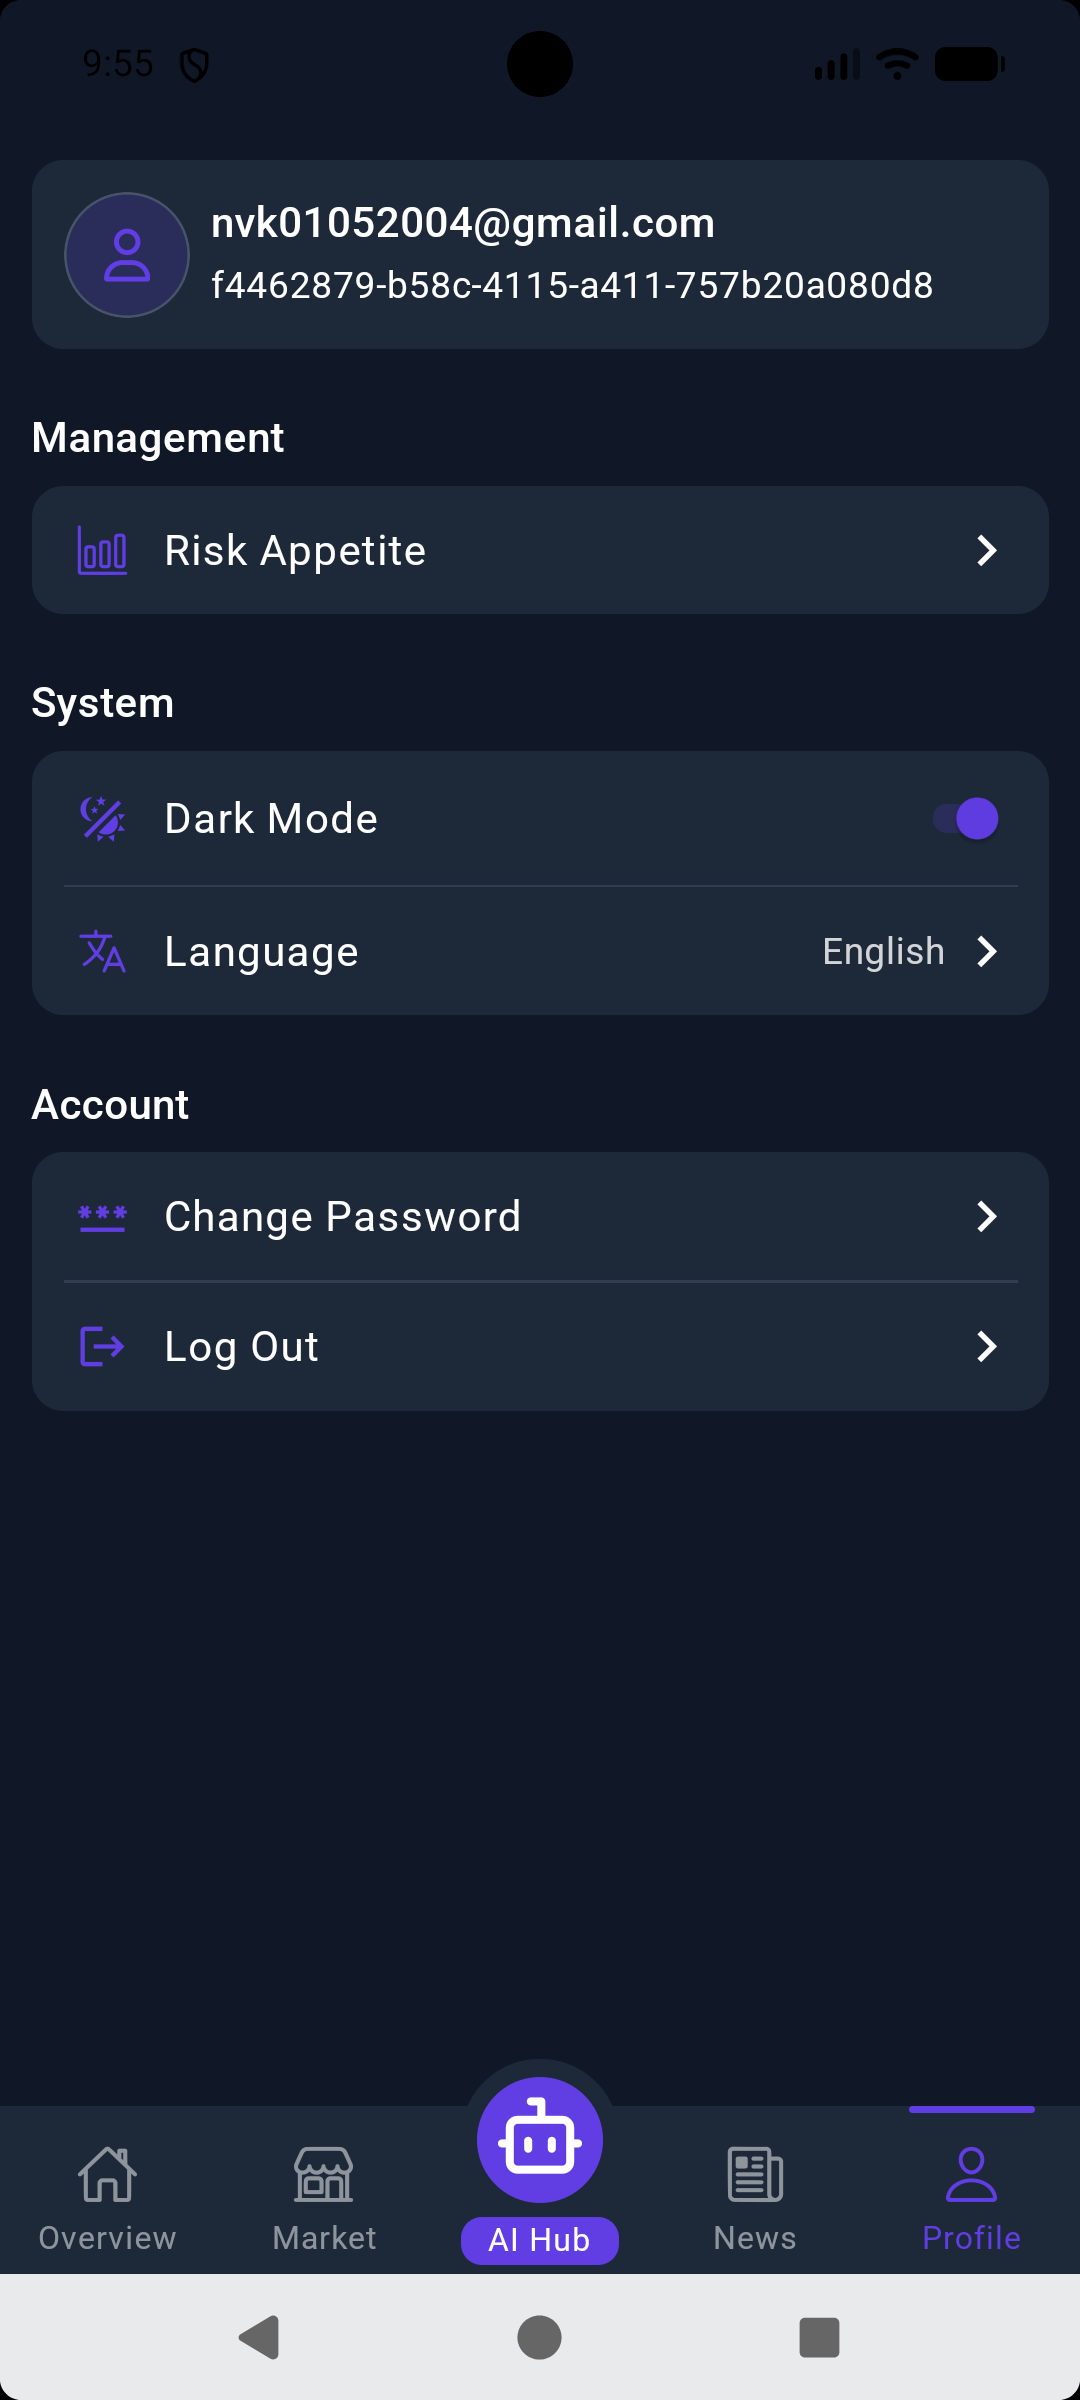
\includegraphics[width=\linewidth]{screenshots/account3.png}\\[2pt]
        \footnotesize (c) Profile screen
    \end{minipage}
    \caption{Authentication and account management interfaces}
    \label{fig:stockrium-captures1}
\end{figure}

In Figure~\ref{fig:stockrium-captures1}(a), users can sign in with an email address and password, use Google authentication, switch to registration, or start password recovery. Figure~\ref{fig:stockrium-captures1}(b) presents the personal watchlist with each saved symbol's latest price and intraday change and provides access to stock search and detail views. Figure~\ref{fig:stockrium-captures1}(c) centralizes profile and preference management, including investment horizon, theme, language, password changes, and logout.

\section{Market Overview and Stock Discovery Demo}
\label{sec:demo-market-discovery}

Figure~\ref{fig:stockrium-captures2} shows the home, market, and search entry points through which an investor discovers securities and opens a stock context.

\begin{figure}[H]
    \centering
    \begin{minipage}[t]{0.32\textwidth}
        \vspace{0pt}
        \centering
        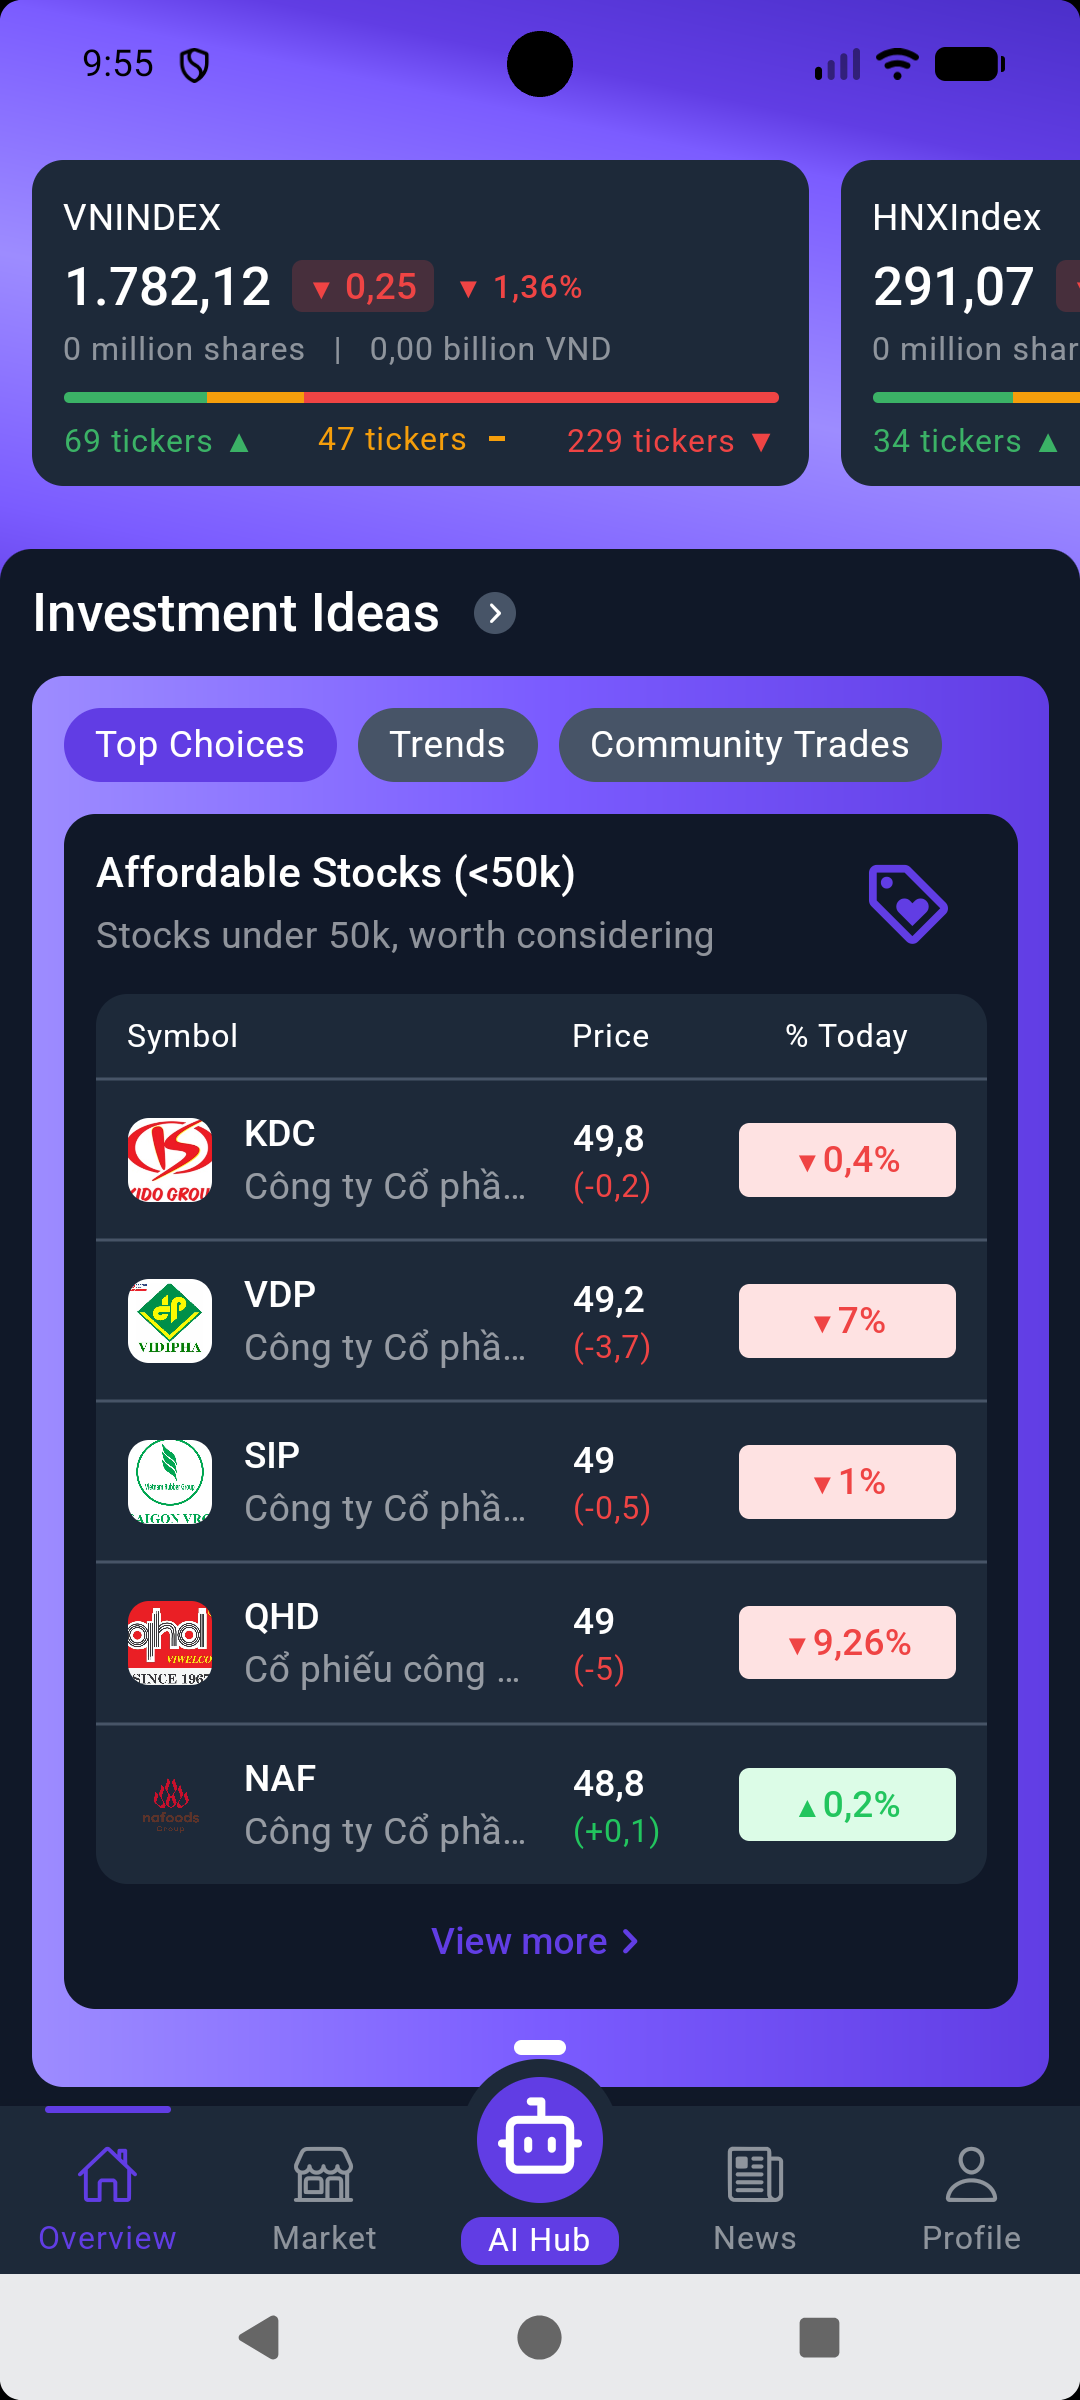
\includegraphics[width=\linewidth]{screenshots/market1.png}\\[2pt]
        \footnotesize (a) Home screen
    \end{minipage}%
    \hfill
    \begin{minipage}[t]{0.32\textwidth}
        \vspace{0pt}
        \centering
        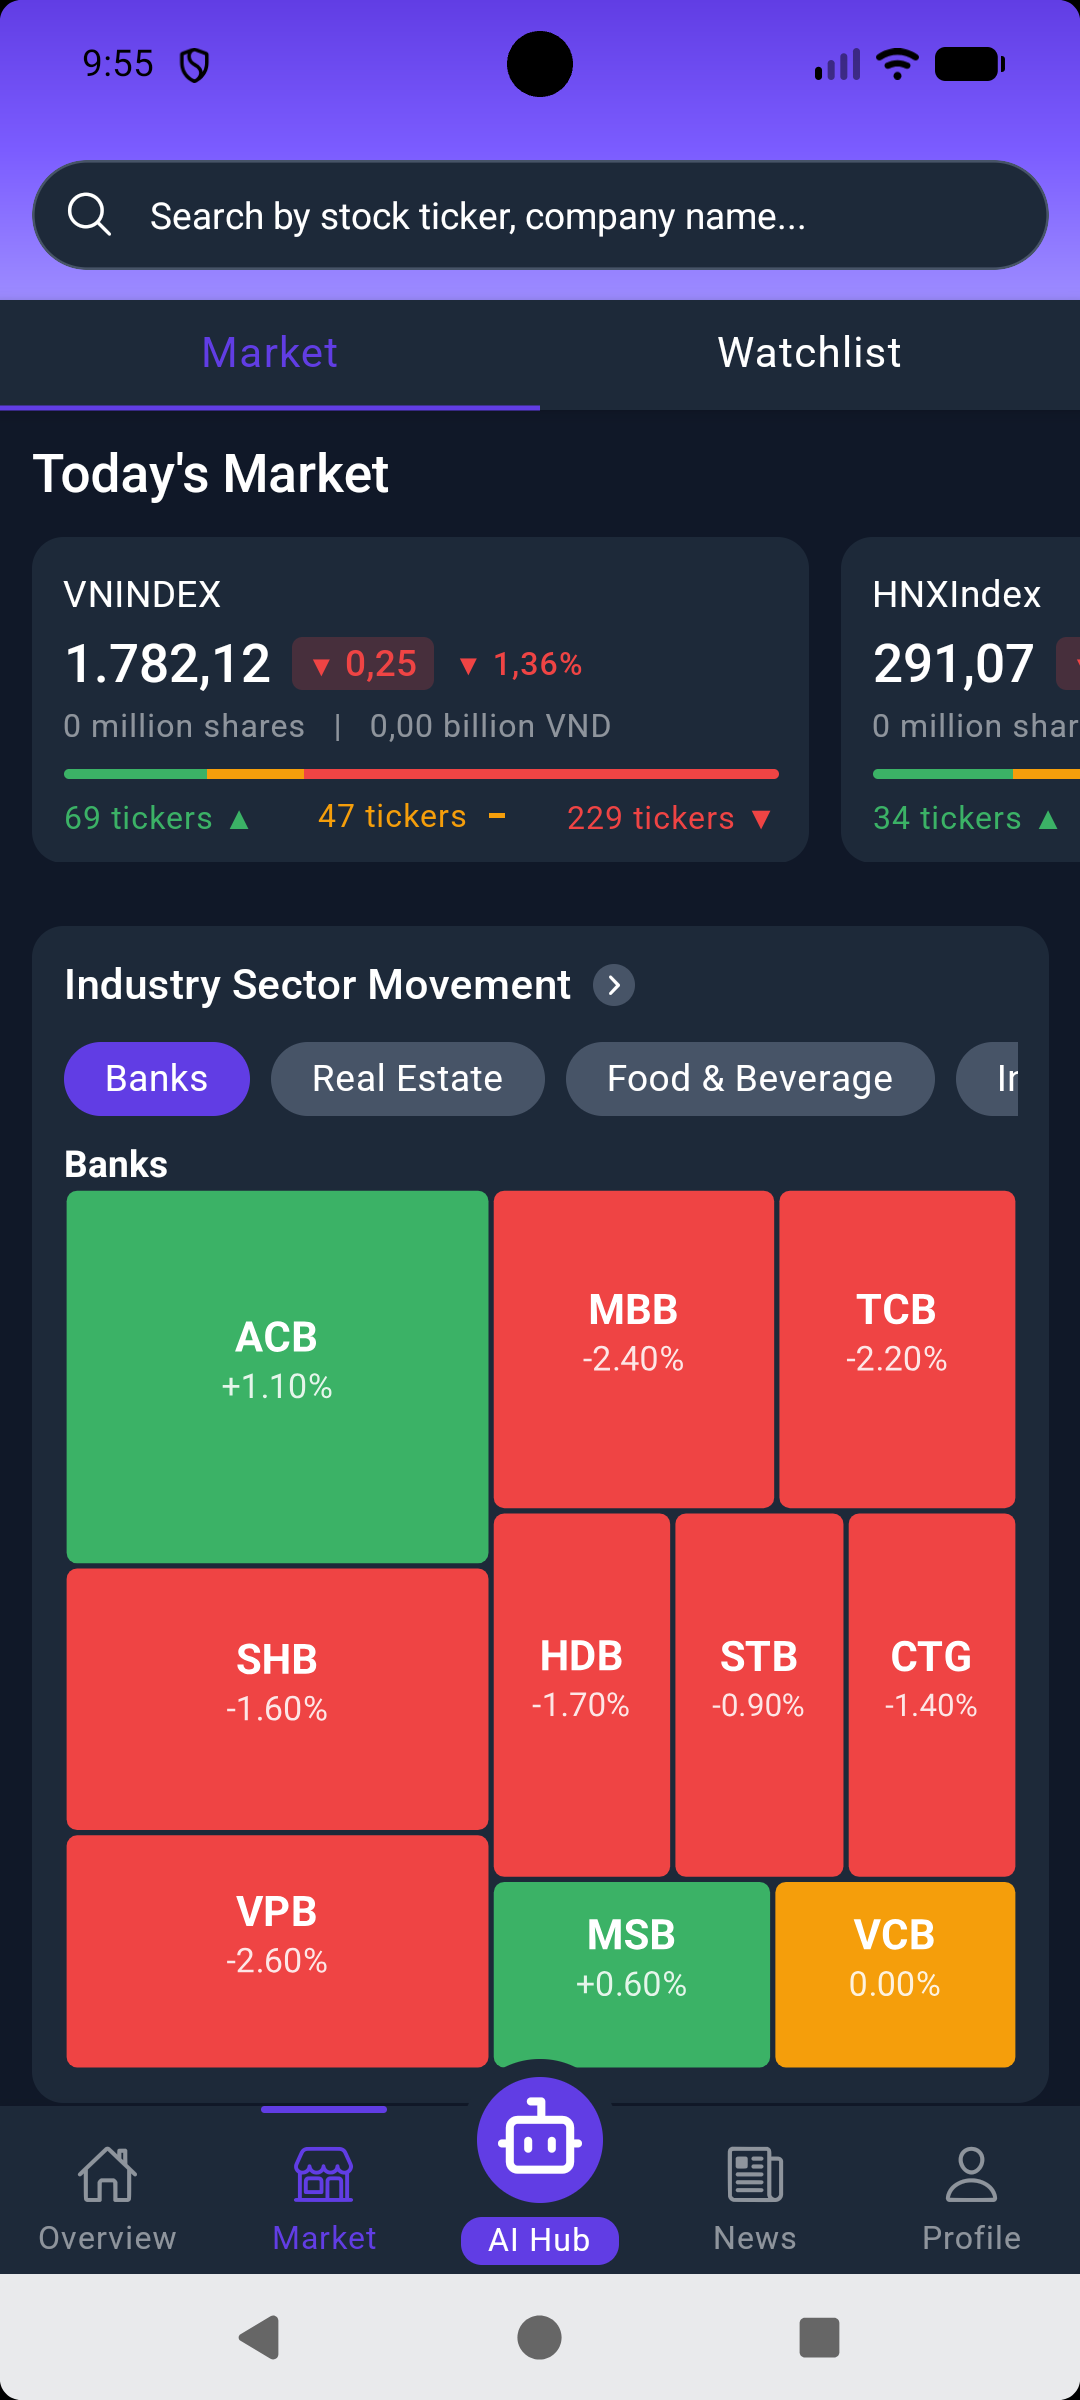
\includegraphics[width=\linewidth]{screenshots/market2.png}\\[2pt]
        \footnotesize (b) Market screen
    \end{minipage}%
    \hfill
    \begin{minipage}[t]{0.32\textwidth}
        \vspace{0pt}
        \centering
        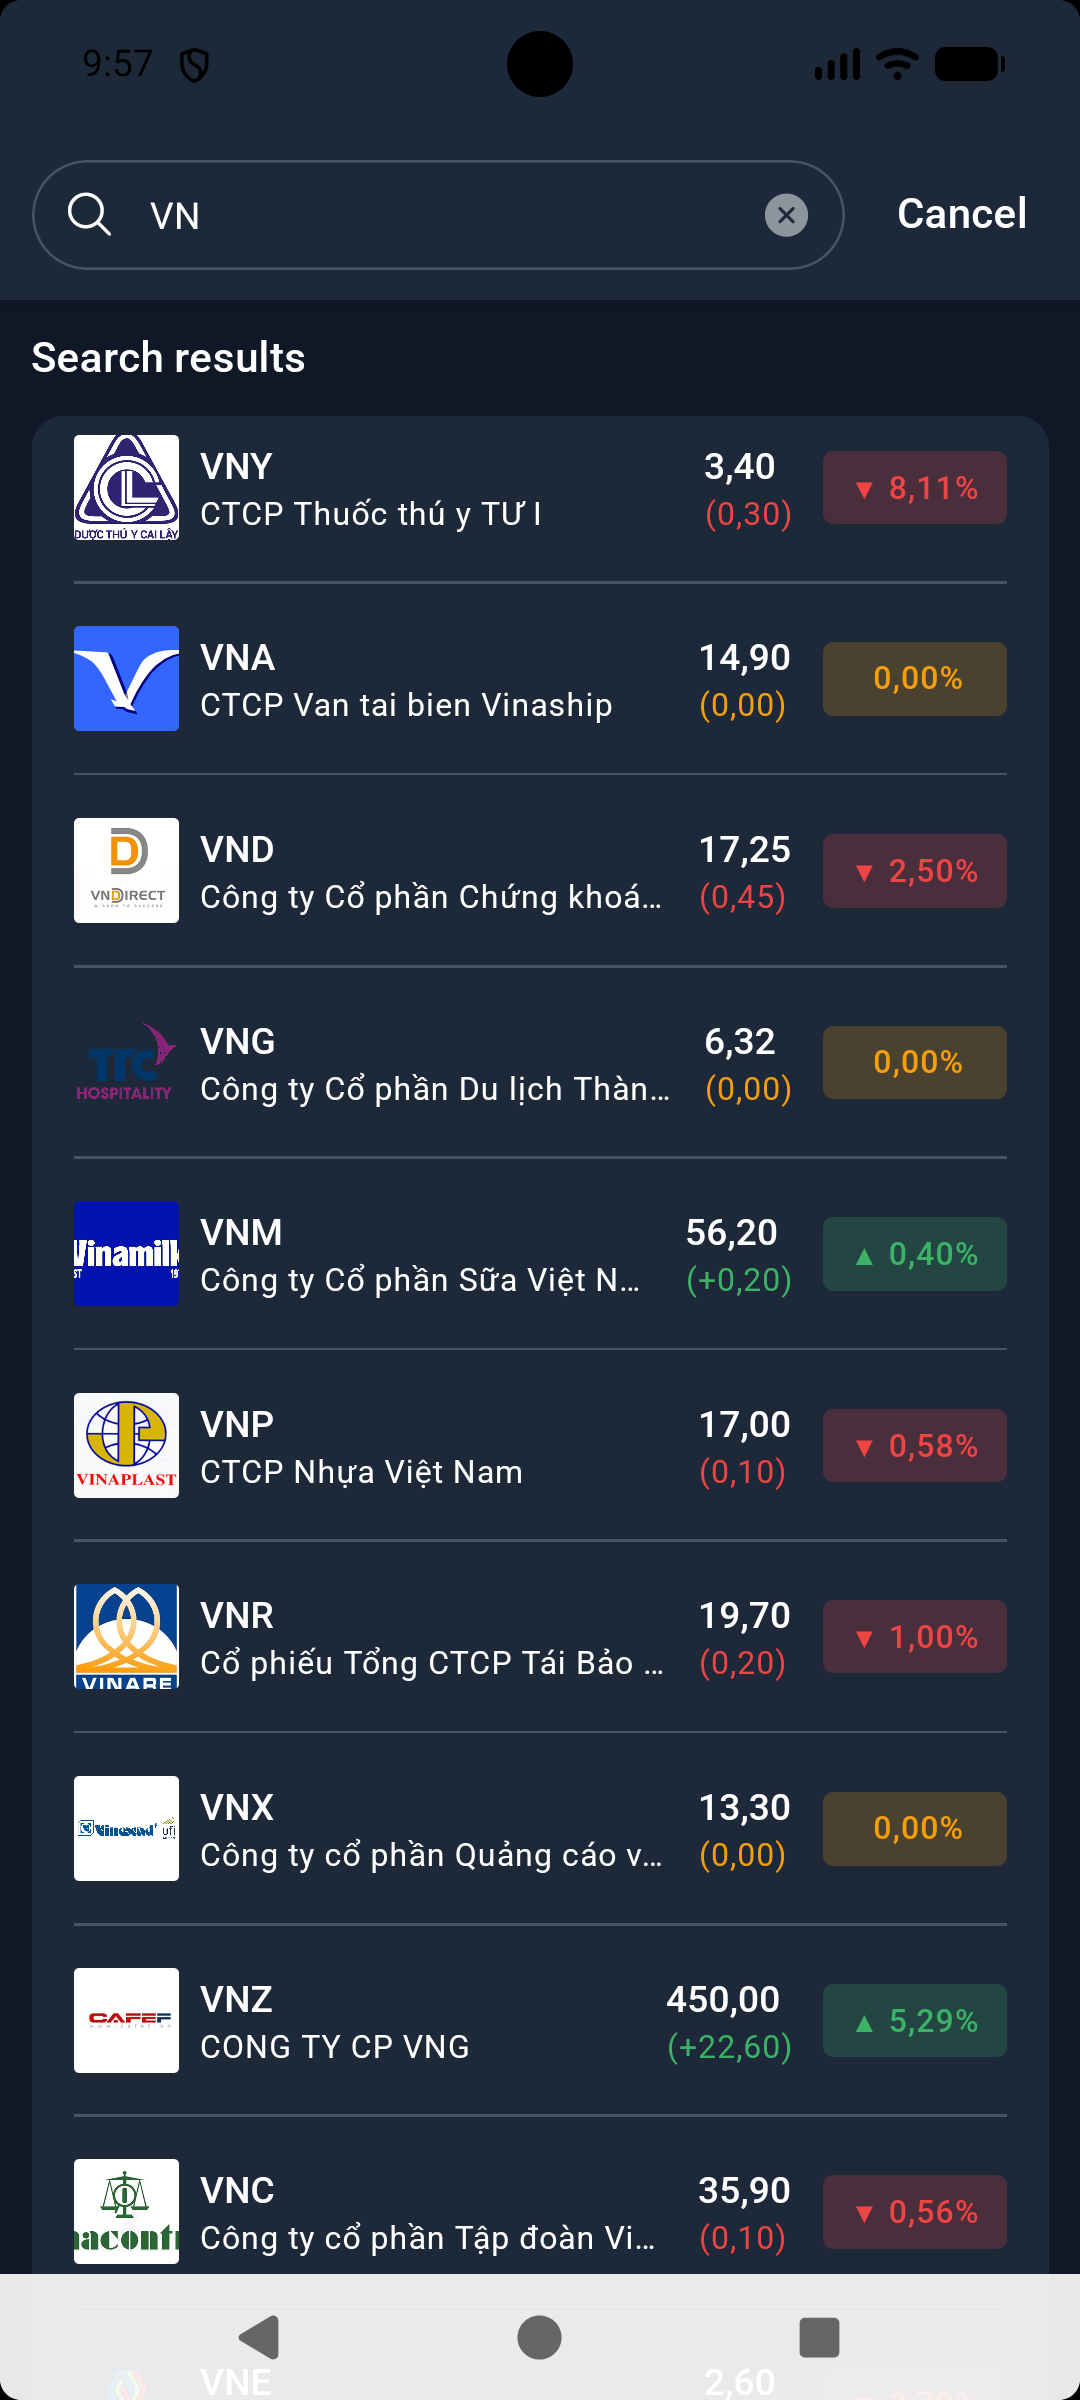
\includegraphics[width=\linewidth]{screenshots/market3.png}\\[2pt]
        \footnotesize (c) Search screen
    \end{minipage}
    \caption{Market overview and stock-discovery interfaces}
    \label{fig:stockrium-captures2}
\end{figure}

Figure~\ref{fig:stockrium-captures2}(a) gives a compact overview of major indices and organizes investment ideas into browsable groups such as top choices, trends, and affordable stocks. Figure~\ref{fig:stockrium-captures2}(b) provides a broader market view with index breadth and an industry heat map so that users can compare sector and stock movements. Figure~\ref{fig:stockrium-captures2}(c) supports lookup by ticker or company name and returns matching securities with their current prices and intraday changes; selecting a result opens the corresponding stock-detail context.

\section{Stock Details and Technical Charts Demo}
\label{sec:demo-stock-details}

Figure~\ref{fig:stockrium-captures3} demonstrates the stock-detail views used to inspect price behavior, technical charts, company information, and financial evidence.

\begin{figure}[H]
    \centering
    \begin{minipage}[t]{0.32\textwidth}
        \vspace{0pt}
        \centering
        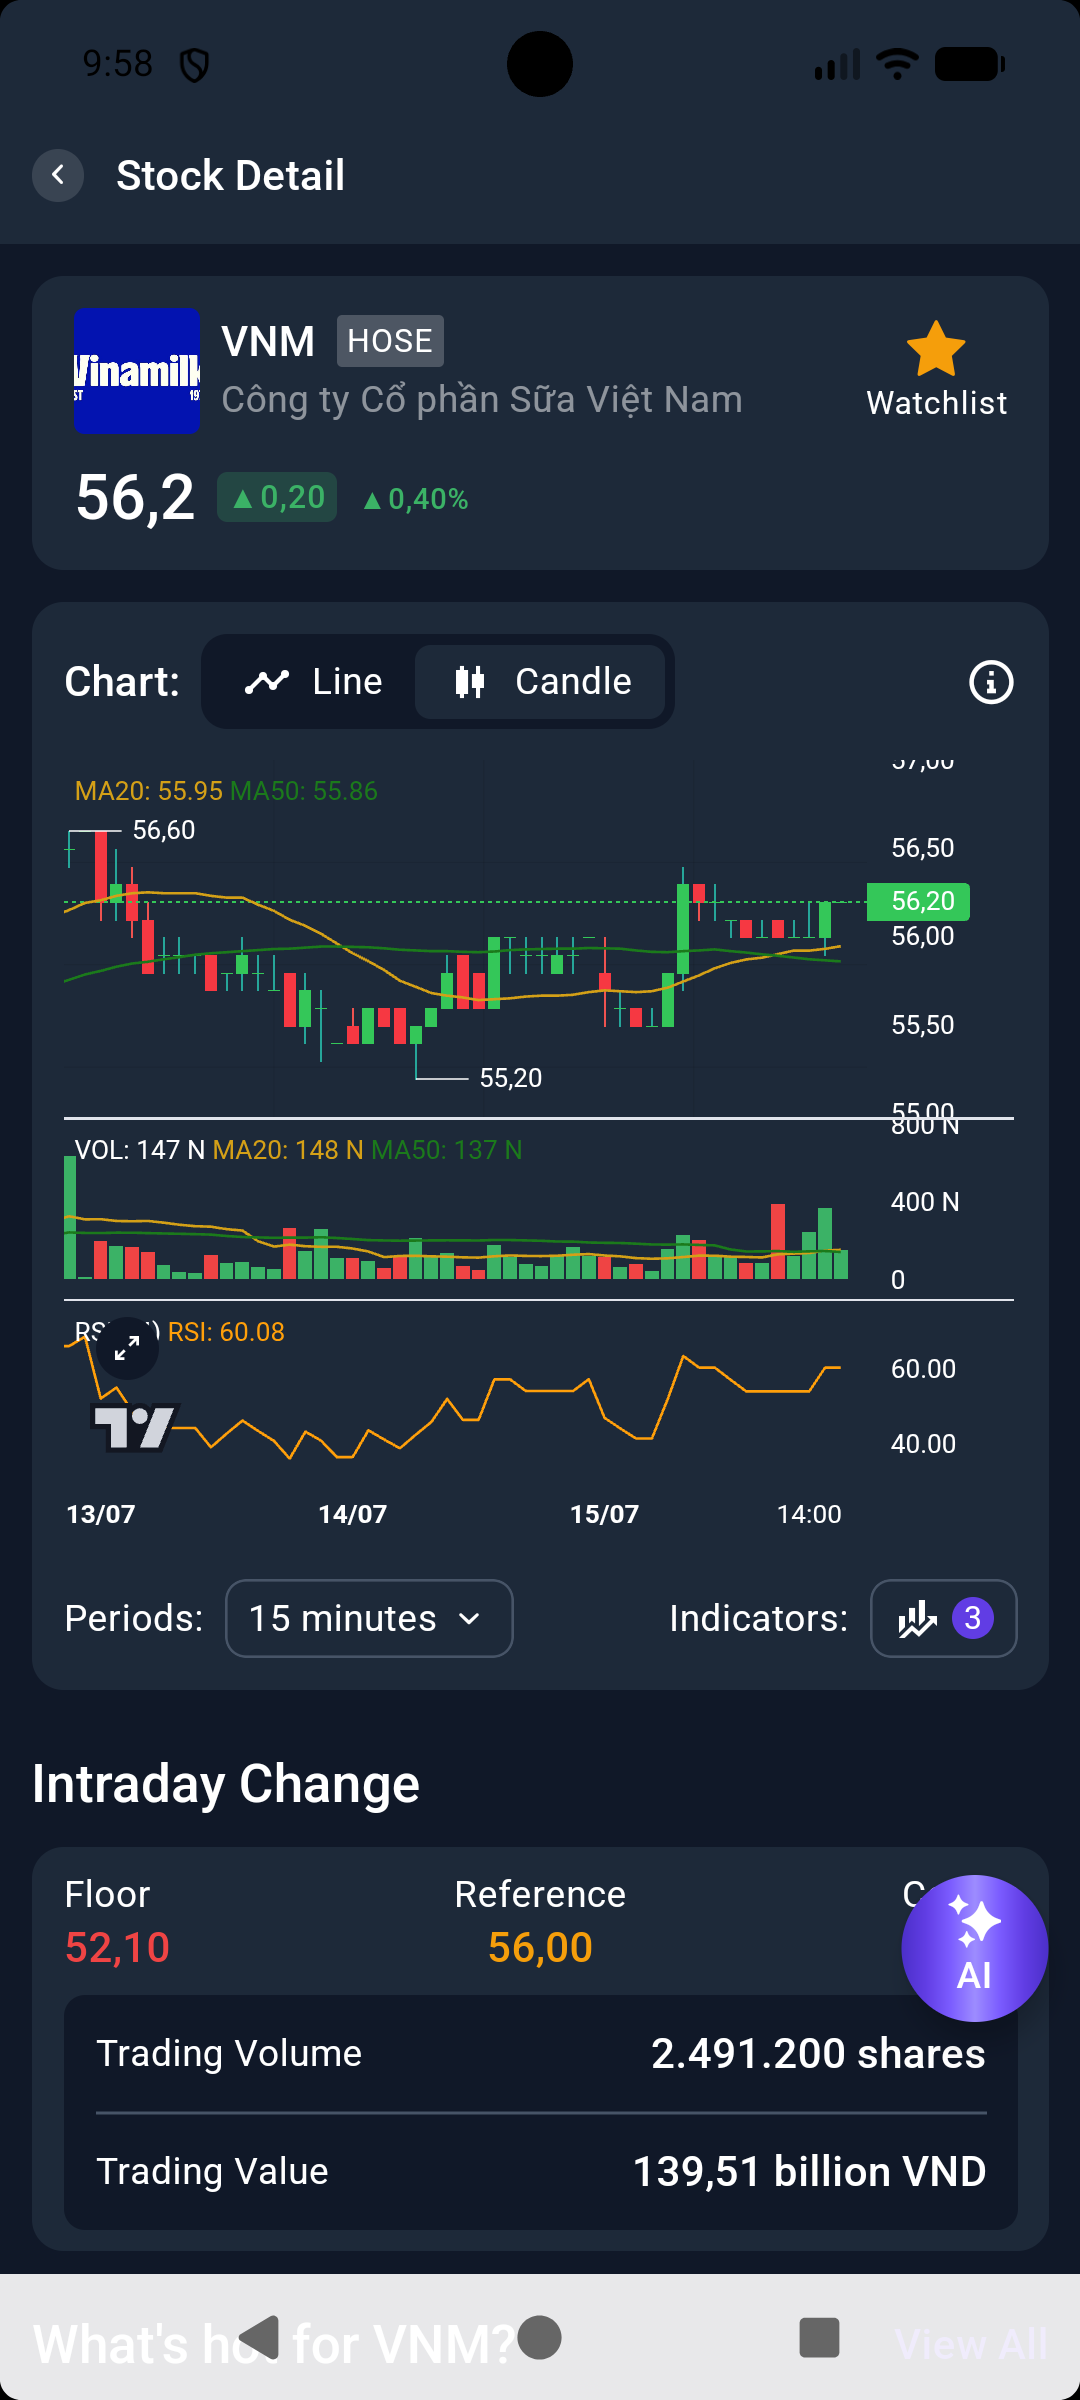
\includegraphics[width=\linewidth]{screenshots/detail1.png}\\[2pt]
        \footnotesize (a) Price and technical-chart view
    \end{minipage}%
    \hfill
    \begin{minipage}[t]{0.32\textwidth}
        \vspace{0pt}
        \centering
        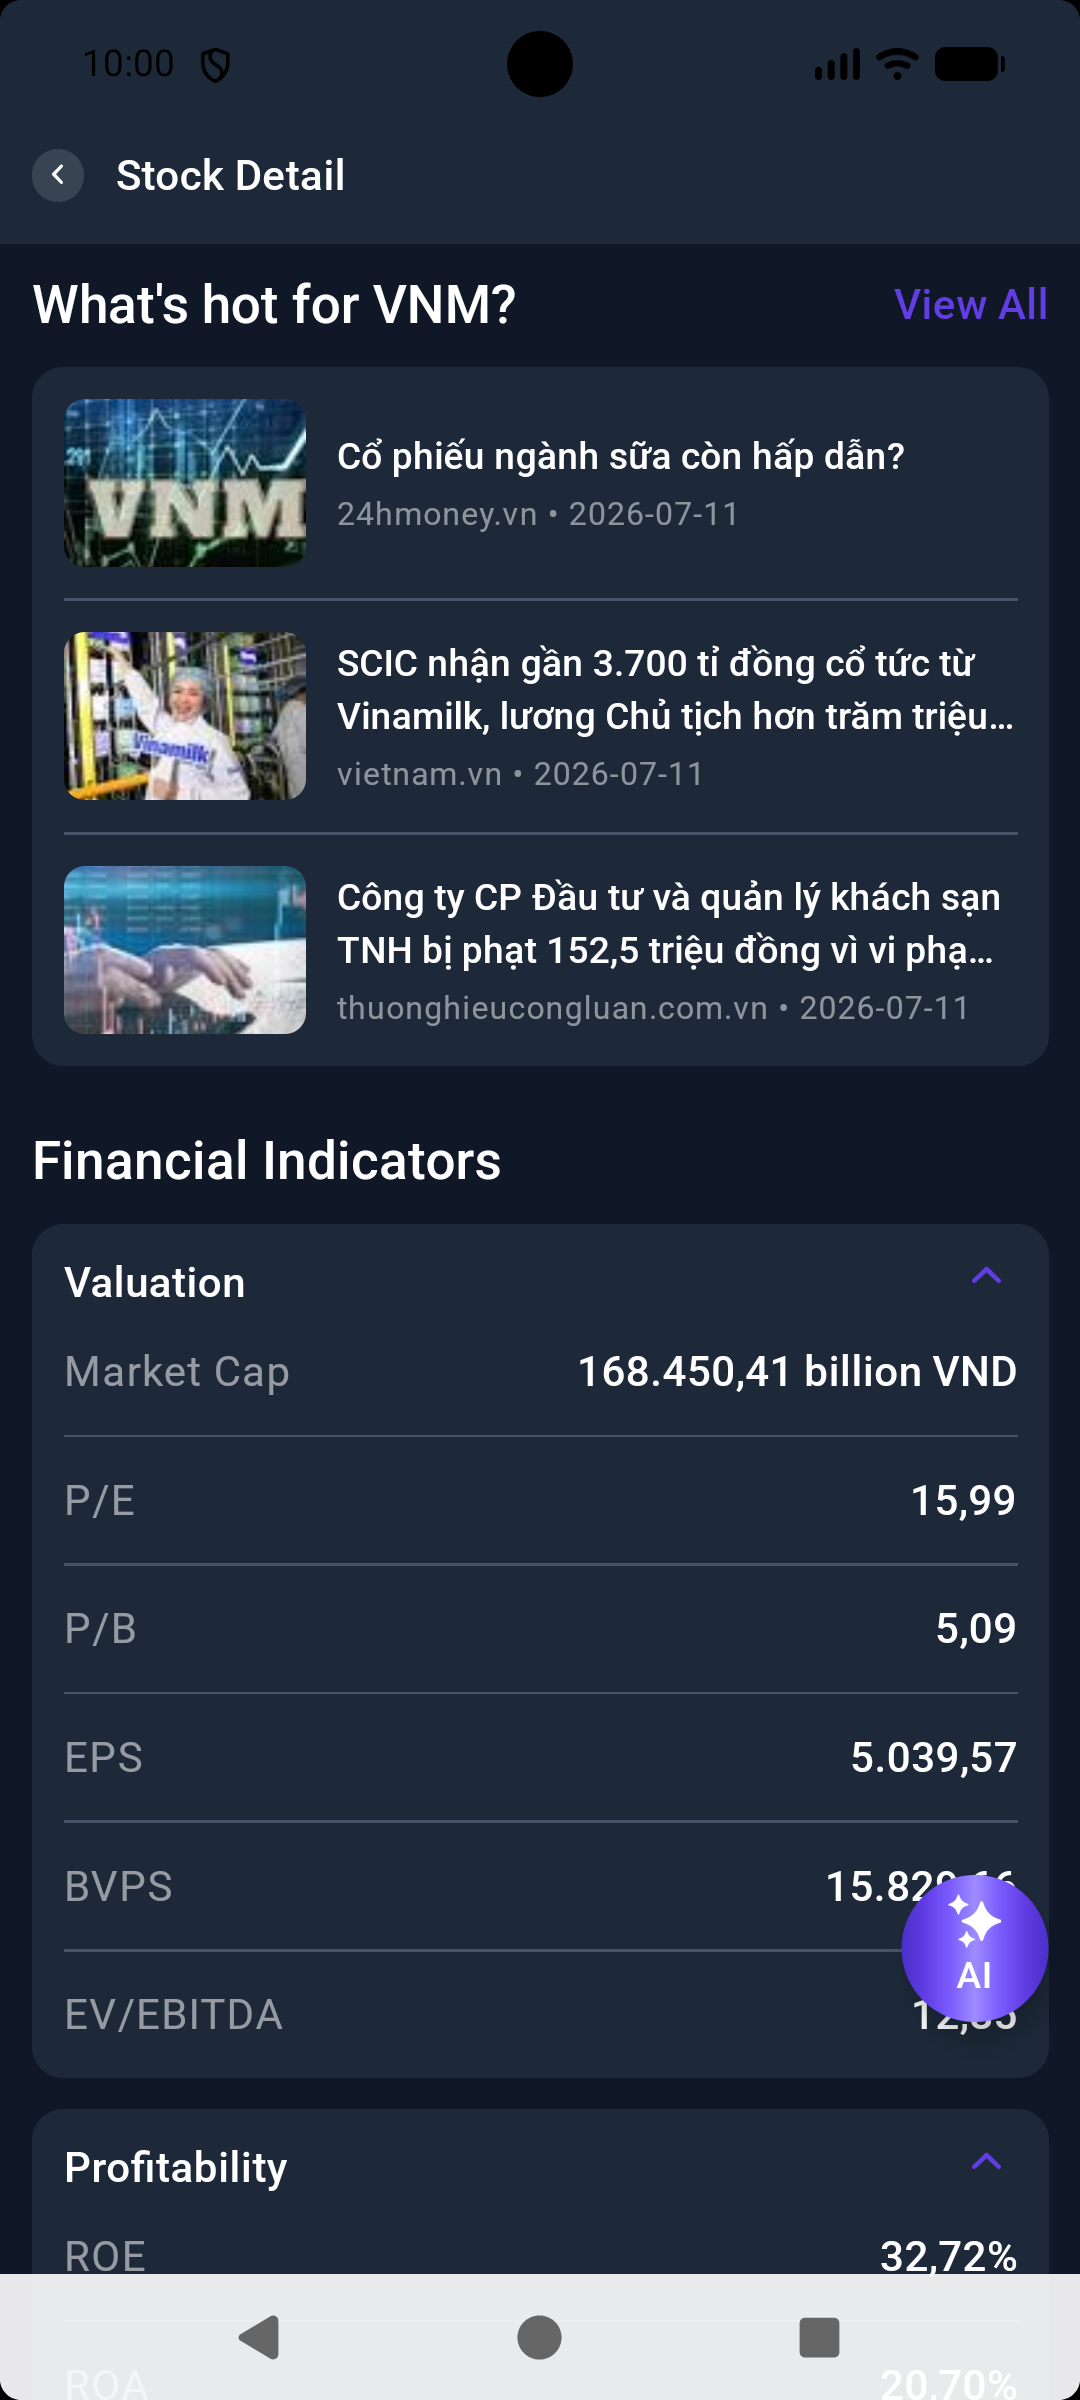
\includegraphics[width=\linewidth]{screenshots/detail2.png}\\[2pt]
        \footnotesize (b) Related news and financial ratios
    \end{minipage}%
    \hfill
    \begin{minipage}[t]{0.32\textwidth}
        \vspace{0pt}
        \centering
        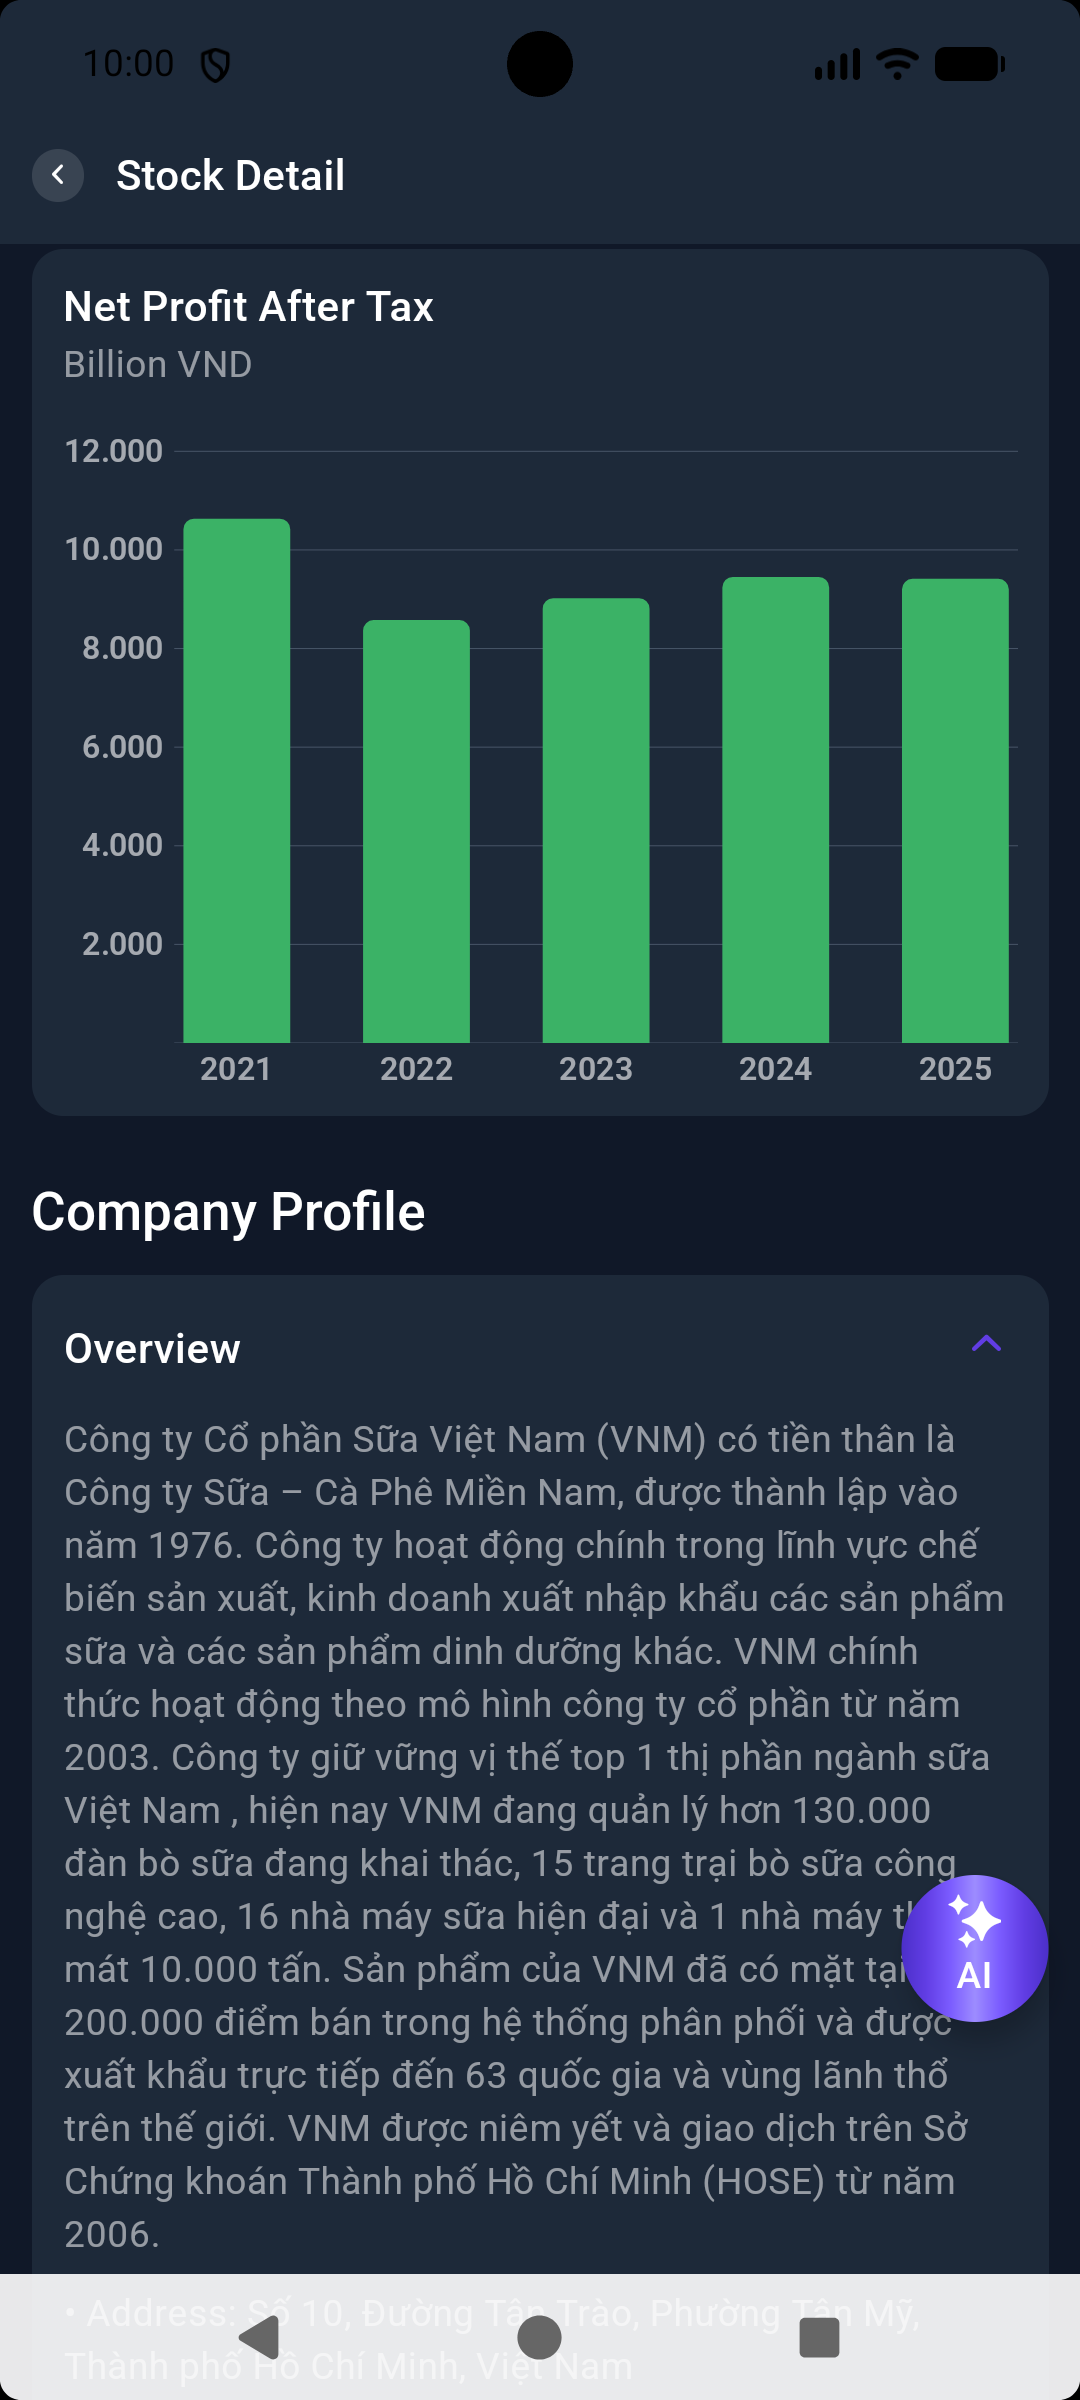
\includegraphics[width=\linewidth]{screenshots/detail3.png}\\[2pt]
        \footnotesize (c) Financial history and company profile
    \end{minipage}
    \caption{Stock-detail evidence views}
    \label{fig:stockrium-captures3}
\end{figure}

Figure~\ref{fig:stockrium-captures3}(a) displays the selected stock's current price, watchlist state, line or candlestick chart, interval controls, volume, technical indicators, and intraday trading information. Figure~\ref{fig:stockrium-captures3}(b) connects recent company-related articles with valuation, profitability, liquidity, leverage, and other financial indicators. Figure~\ref{fig:stockrium-captures3}(c) presents historical financial performance together with the company profile. These views keep price action, technical evidence, relevant news, financial ratios, historical performance, and company information within the same stock context, allowing the investor to cross-check the evidence before opening the multi-agent workflow.

\section{Financial News Demo}
\label{sec:demo-financial-news}

Figure~\ref{fig:stockrium-captures4} presents the financial-news collections and article-detail interface, including the processed information available to the investor.

\begin{figure}[H]
    \centering
    \begin{minipage}[t]{0.32\textwidth}
        \vspace{0pt}
        \centering
        
\includegraphics[width=\linewidth]{screenshots/news1.png}\\[2pt]
        \footnotesize (a) News collection
    \end{minipage}%
    \hfill
    \begin{minipage}[t]{0.32\textwidth}
        \vspace{0pt}
        \centering
        
\includegraphics[width=\linewidth]{screenshots/news2.png}\\[2pt]
        \footnotesize (b) News category
    \end{minipage}%
    \hfill
    \begin{minipage}[t]{0.32\textwidth}
        \vspace{0pt}
        \centering
        
\includegraphics[width=\linewidth]{screenshots/news3.png}\\[2pt]
        \footnotesize (c) Article details
    \end{minipage}
    \caption{Financial-news exploration interfaces}
    \label{fig:stockrium-captures4}
\end{figure}

Figure~\ref{fig:stockrium-captures4}(a) combines daily highlights with general business-news collections and provides direct navigation to selected stories. Figure~\ref{fig:stockrium-captures4}(b) groups articles by industry and also exposes economy and macroeconomic collections, enabling users to narrow the information space before opening an article. Figure~\ref{fig:stockrium-captures4}(c) displays the selected article's title, publisher, publication date, processed summary, and full content for detailed reading.

\section{Configurable Multi-Agent Analysis Demo}
\label{sec:demo-multi-agent-analysis}

Figure~\ref{fig:stockrium-captures5} shows the investment-horizon and manual-configuration inputs. Figure~\ref{fig:stockrium-captures6} shows the structured assessment and its supporting analytical results.

\begin{figure}[H]
    \centering
    \begin{minipage}[t]{0.45\textwidth}
        \vspace{0pt}
        \centering
        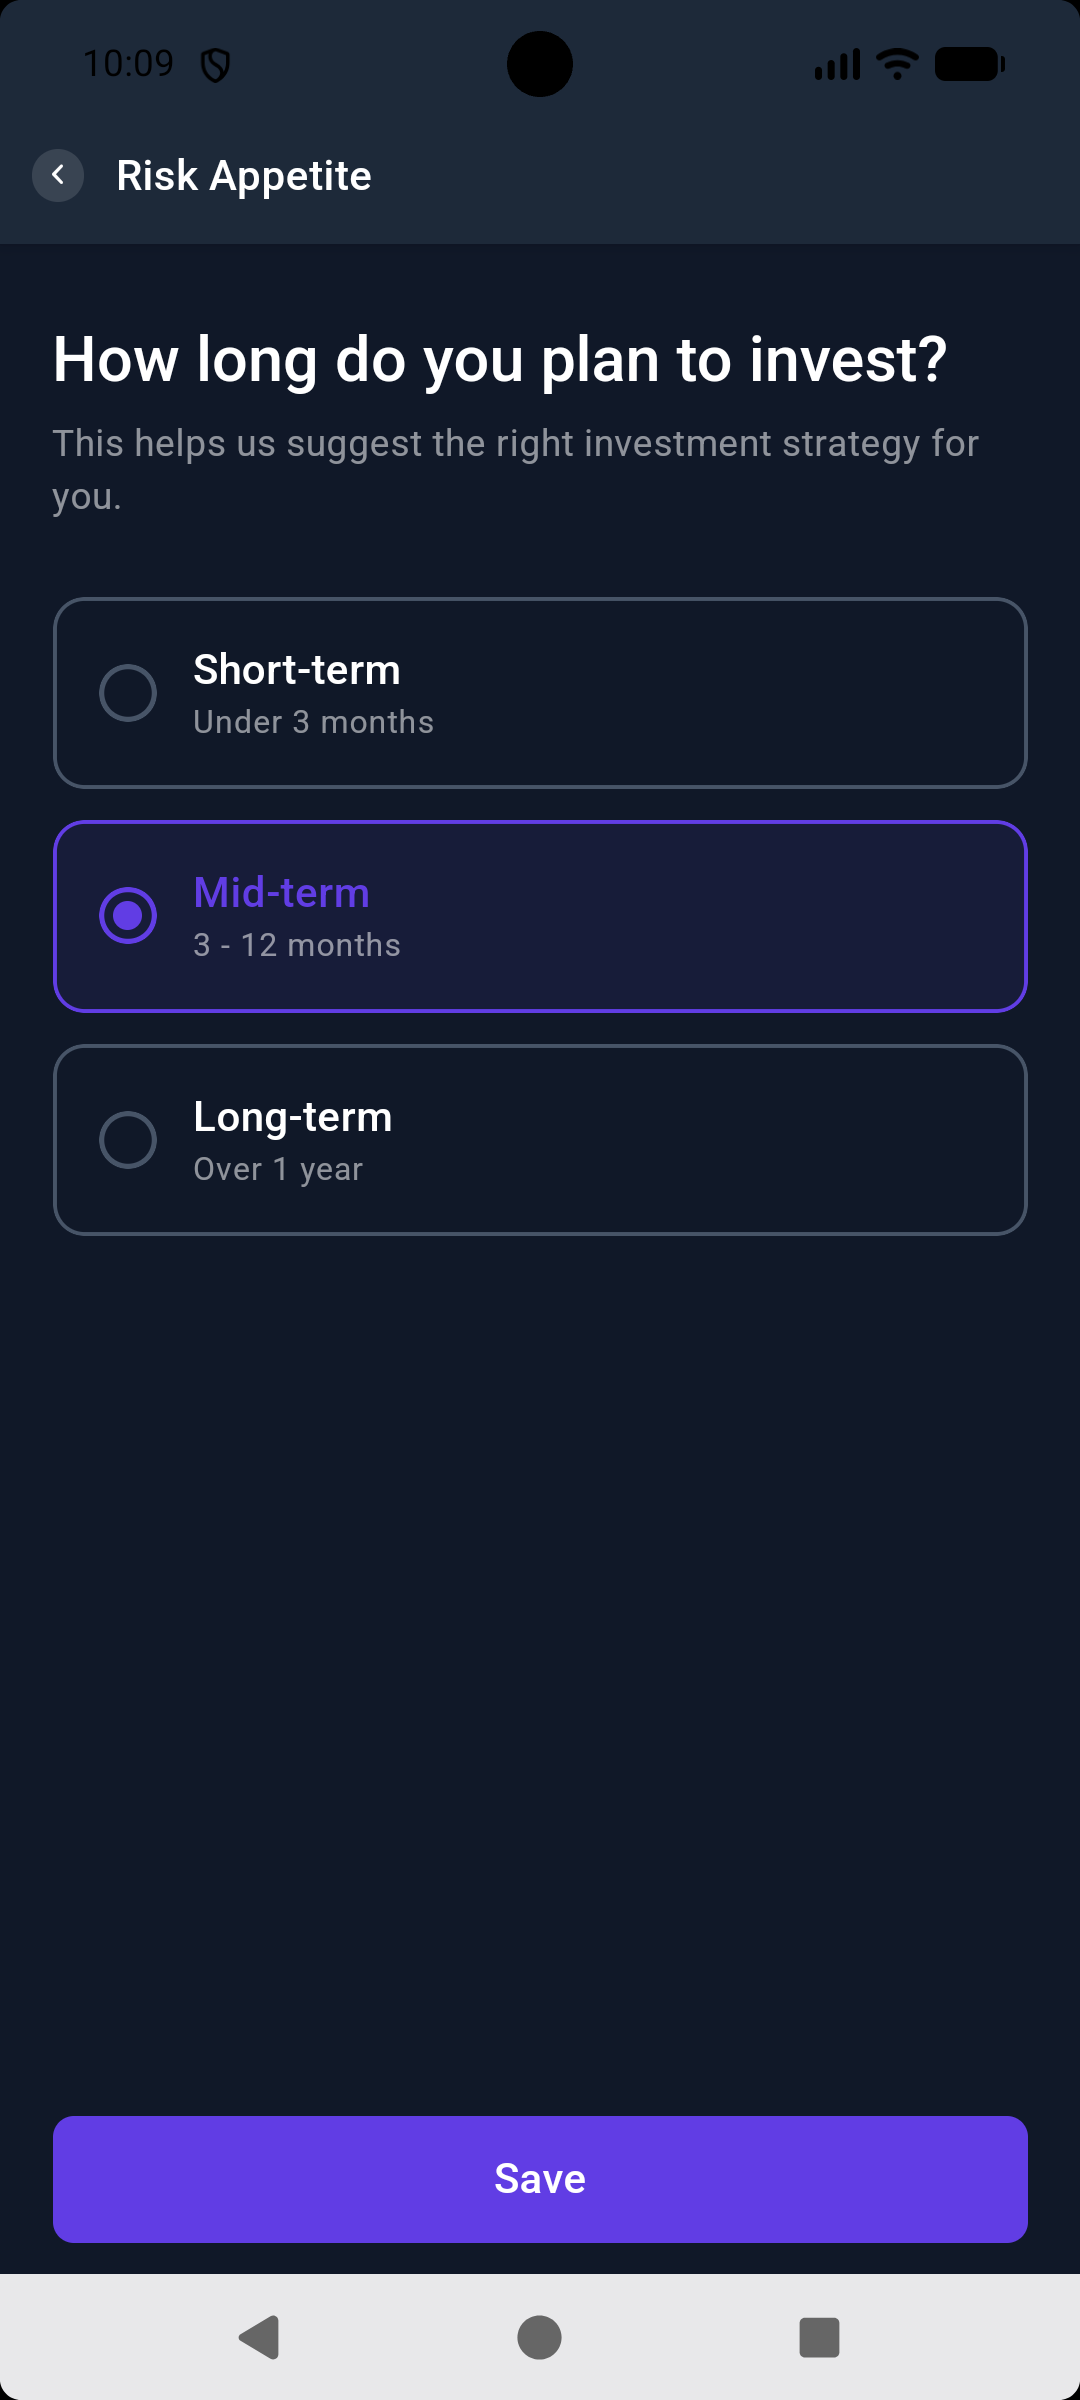
\includegraphics[width=\linewidth]{screenshots/AI1.png}\\[2pt]
        \footnotesize (a) Investment-horizon profile
    \end{minipage}%
    \hspace{1cm}%
    \begin{minipage}[t]{0.45\textwidth}
        \vspace{0pt}
        \centering
        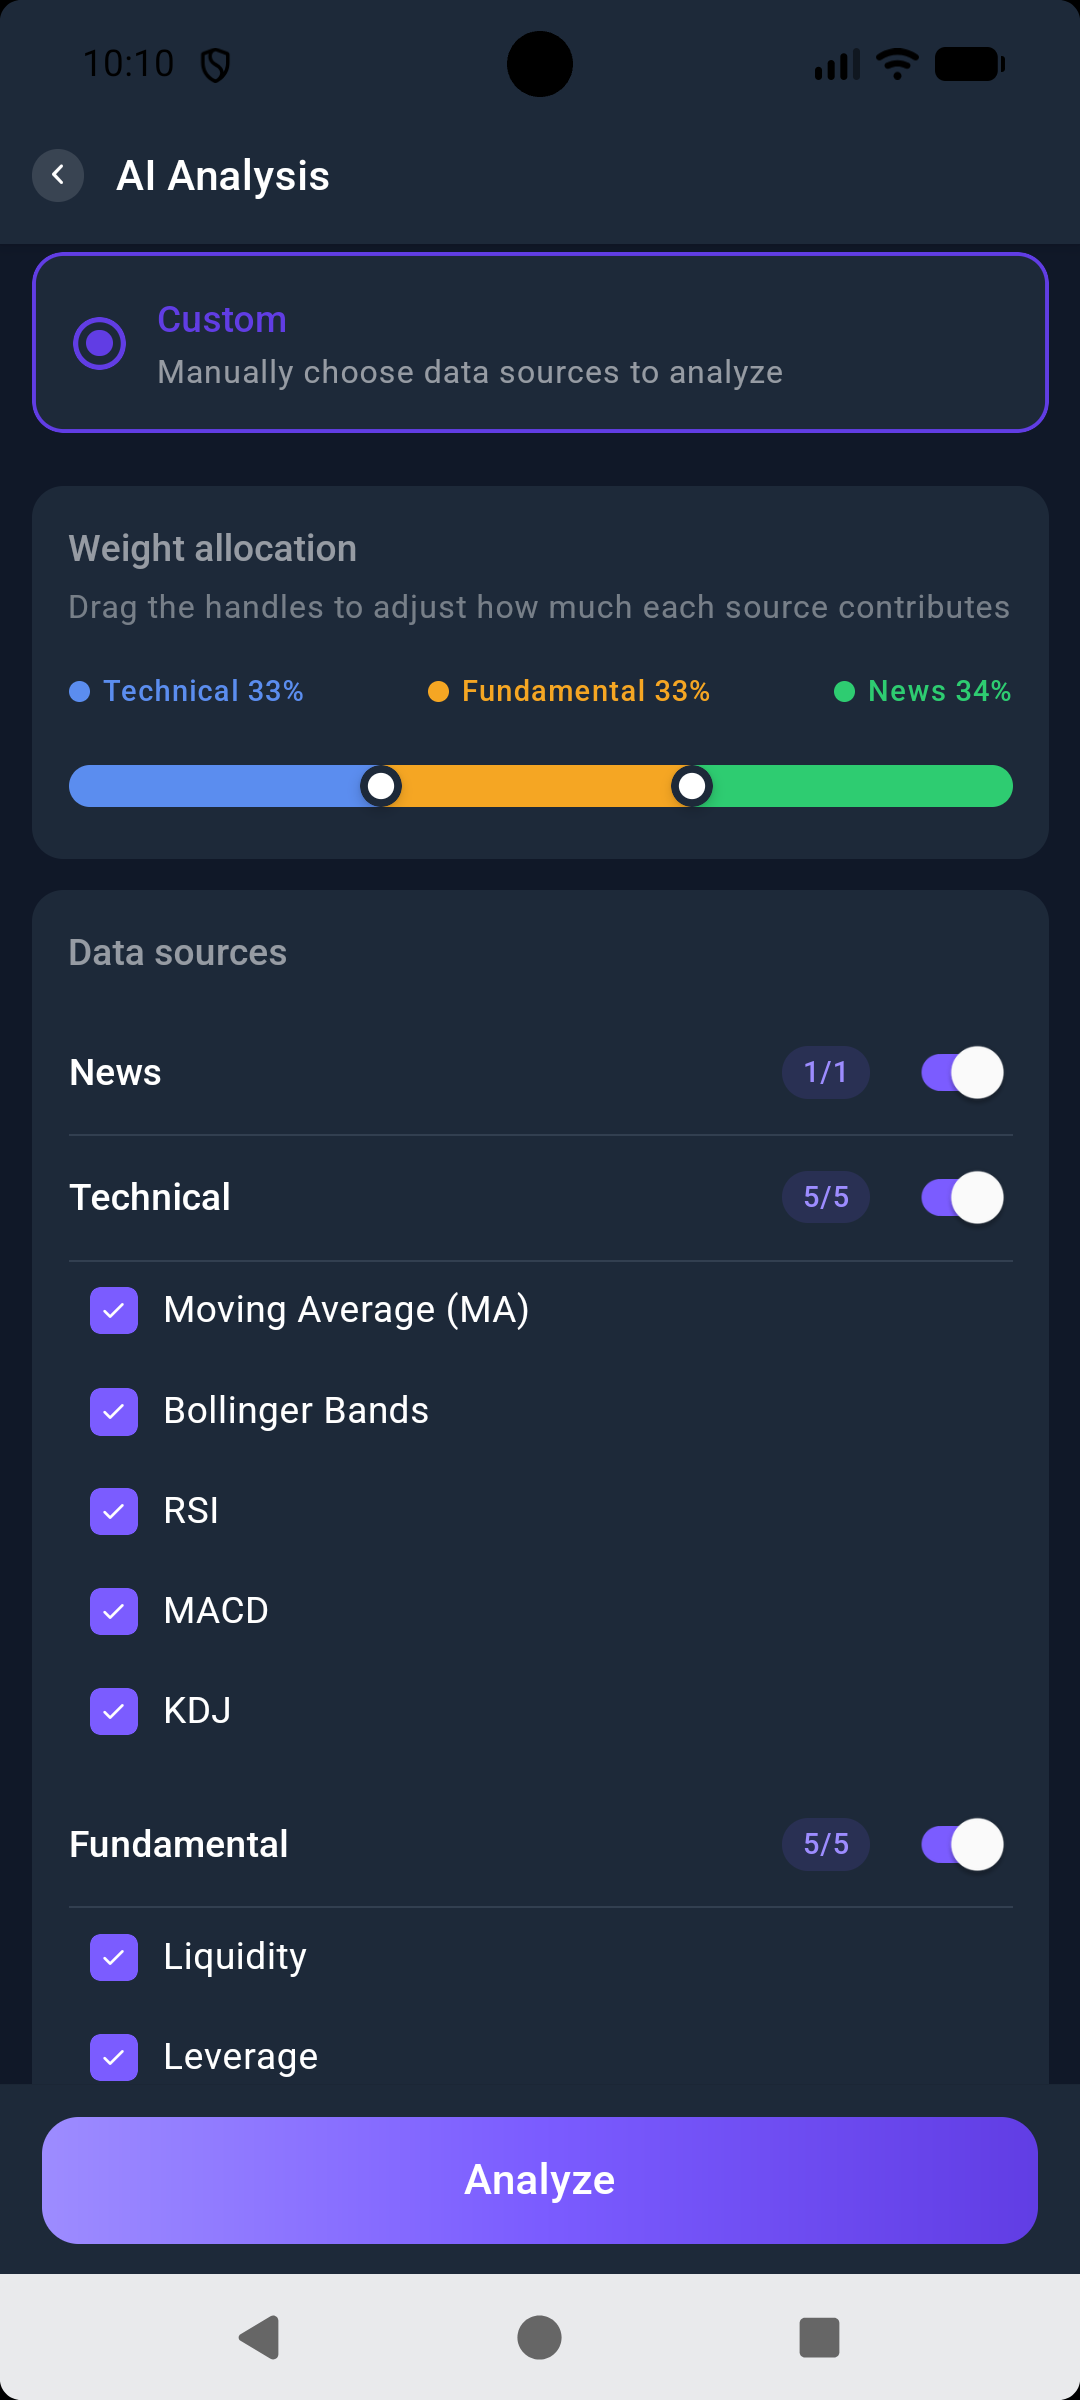
\includegraphics[width=\linewidth]{screenshots/AI2.png}\\[2pt]
        \footnotesize (b) Manual analysis configuration
    \end{minipage}
    \caption{Inputs for configurable multi-agent analysis}
    \label{fig:stockrium-captures5}
\end{figure}

Figure~\ref{fig:stockrium-captures5}(a) allows users to select a short-, medium-, or long-term investment horizon, which determines the preset evidence windows, weights, and trading-plan parameters used in automatic mode. Figure~\ref{fig:stockrium-captures5}(b) supports manual configuration through analytical-source switches, normalized technical, fundamental, and news weights, and technical-indicator selection. In the implemented pipeline, fundamental and news analysis remain whole-source inputs.

\begin{figure}[H]
    \centering
    \begin{minipage}[t]{0.45\textwidth}
        \vspace{0pt}
        \centering
        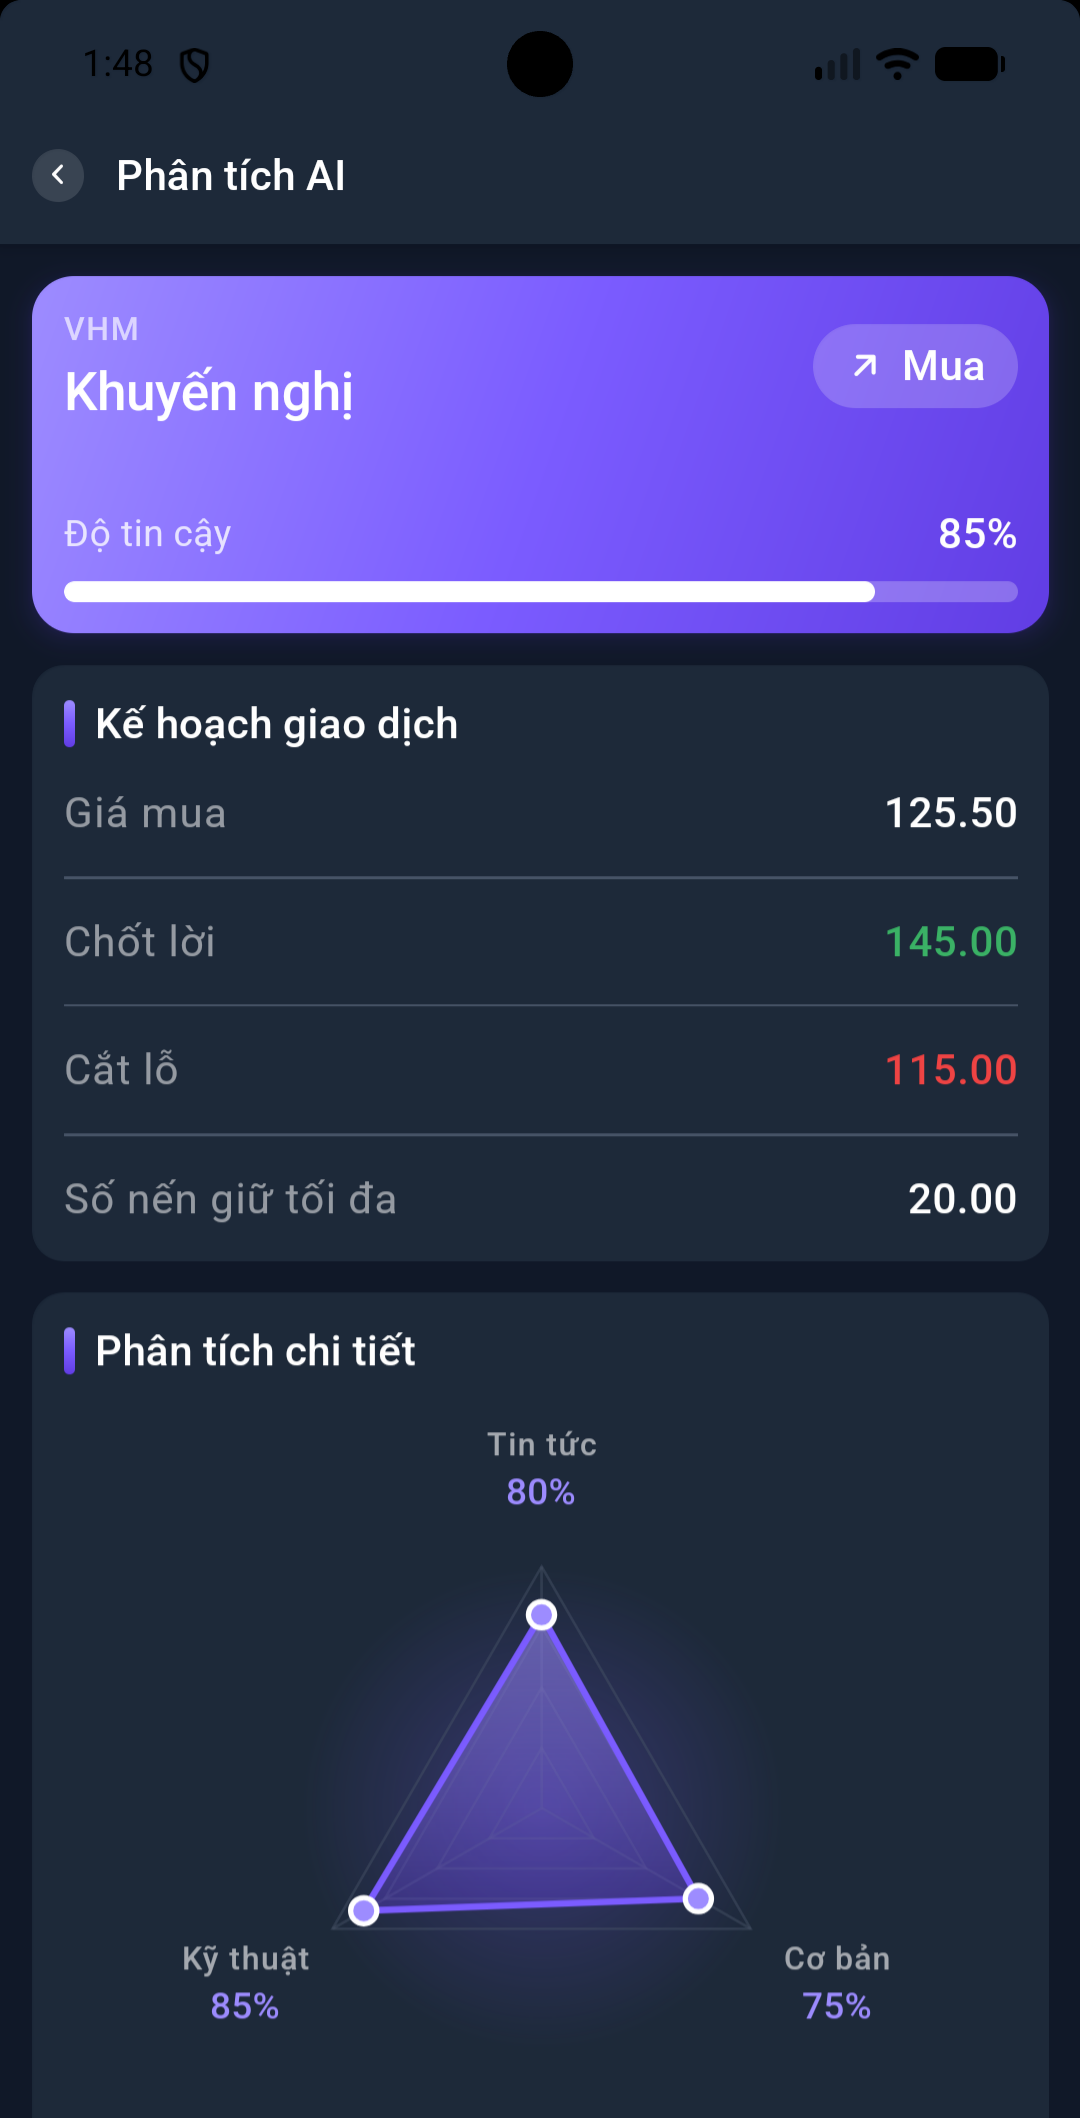
\includegraphics[width=\linewidth]{screenshots/AI3.png}\\[2pt]
        \footnotesize (a) Assessment overview
    \end{minipage}%
    \hspace{1cm}%
    \begin{minipage}[t]{0.45\textwidth}
        \vspace{0pt}
        \centering
        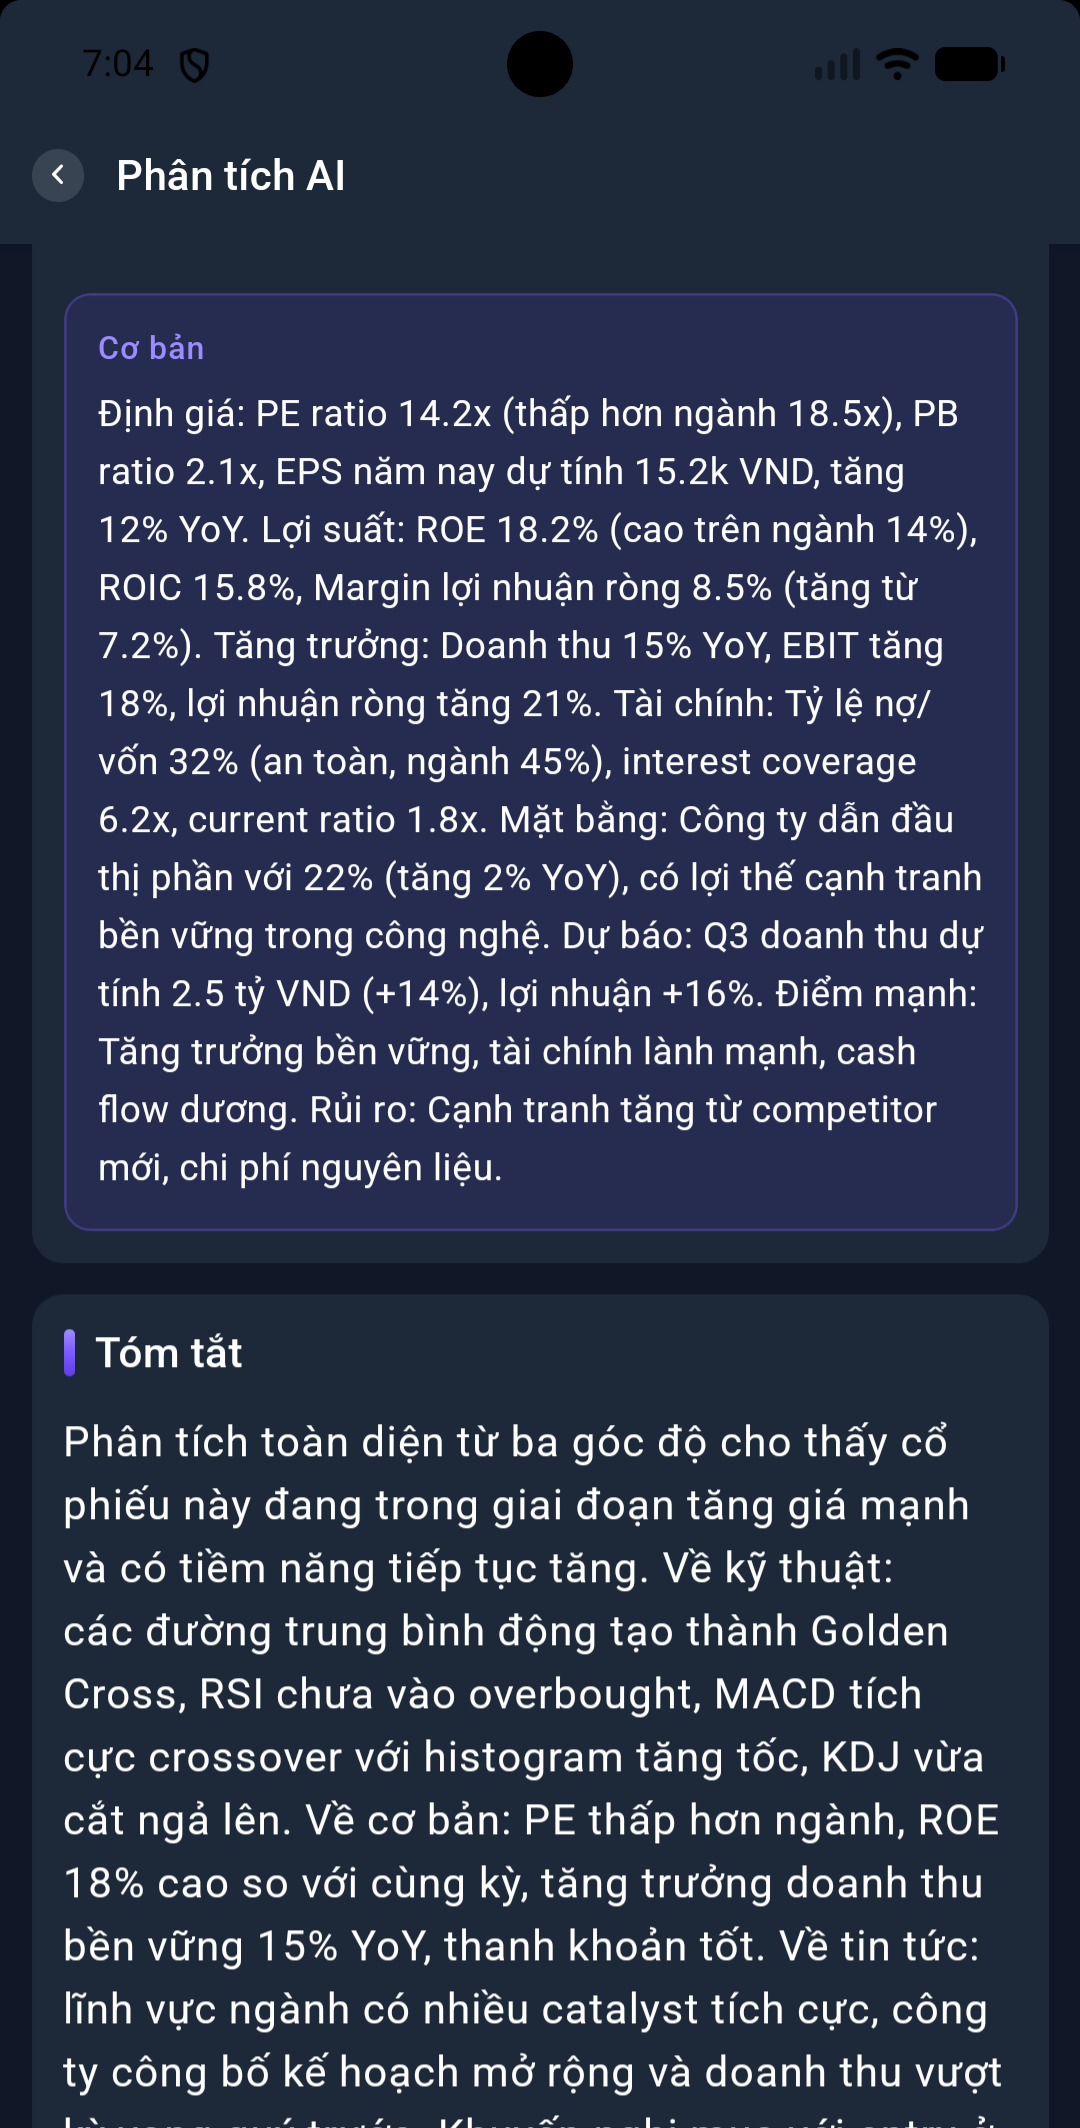
\includegraphics[width=\linewidth]{screenshots/AI4.png}\\[2pt]
        \footnotesize (b) Component evidence and explanation
    \end{minipage}
    \caption{Multi-agent analysis results}
    \label{fig:stockrium-captures6}
\end{figure}

Figure~\ref{fig:stockrium-captures6}(a) summarizes the final Buy-or-Wait assessment, confidence, entry price, take-profit, stop-loss, maximum holding period, and the relative technical, fundamental, and news scores. Figure~\ref{fig:stockrium-captures6}(b) exposes the detailed evidence produced by the specialist agents and the final synthesized explanation. The result view therefore separates the decision and trading-plan fields from their supporting evidence, making each agent's contribution inspectable while keeping confidence as an explanatory decision-support cue rather than a calibrated probability or execution instruction.

\section{Conversational Financial Assistant Demo}
\label{sec:demo-conversational-assistant}

Figure~\ref{fig:stockrium-captures7} demonstrates conversation creation, stored session history, and multi-turn financial interaction.

\begin{figure}[H]
    \centering
    \begin{minipage}[t]{0.32\textwidth}
        \vspace{0pt}
        \centering
        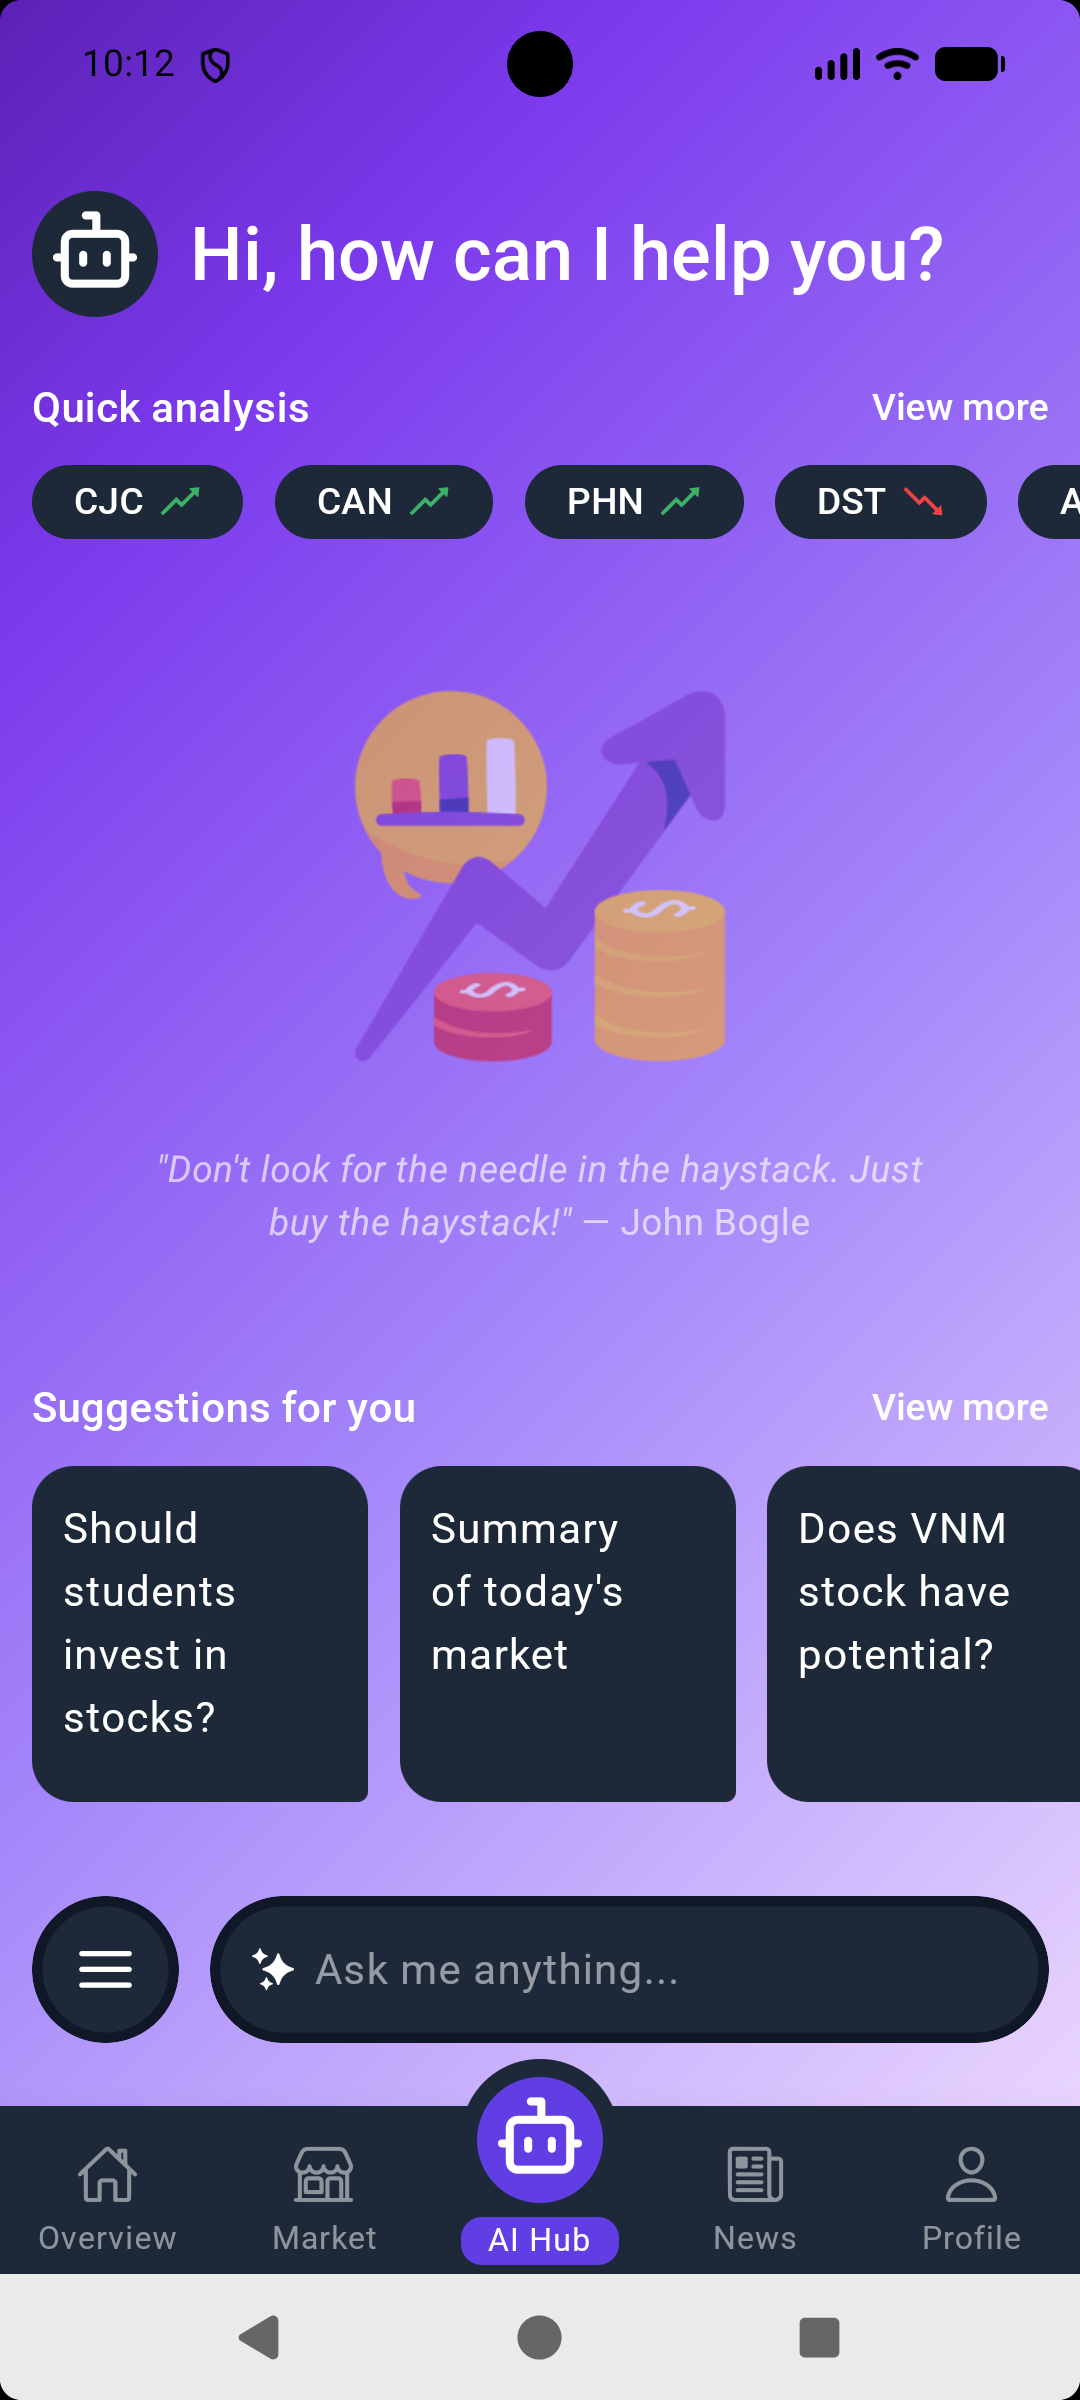
\includegraphics[width=\linewidth]{screenshots/chatbot1.png}\\[2pt]
        \footnotesize (a) Chatbot entry screen
    \end{minipage}%
    \hfill
    \begin{minipage}[t]{0.32\textwidth}
        \vspace{0pt}
        \centering
        
\includegraphics[width=\linewidth]{screenshots/chatbot2.png}\\[2pt]
        \footnotesize (b) Conversation history
    \end{minipage}%
    \hfill
    \begin{minipage}[t]{0.32\textwidth}
        \vspace{0pt}
        \centering
        
\includegraphics[width=\linewidth]{screenshots/chatbot3.png}\\[2pt]
        \footnotesize (c) Conversation screen
    \end{minipage}
    \caption{Conversational financial assistant interfaces}
    \label{fig:stockrium-captures7}
\end{figure}

Figure~\ref{fig:stockrium-captures7}(a) is the chatbot entry point, where users can start with quick stock-analysis shortcuts, suggested financial questions, or a free-form prompt. Figure~\ref{fig:stockrium-captures7}(b) lists saved conversations and supports reopening an earlier session or starting a new one. Figure~\ref{fig:stockrium-captures7}(c) presents the multi-turn conversation view and message composer, allowing the user to continue within the retained session context. The assistant supports general financial exploration, whereas structured stock recommendations remain the responsibility of the configurable multi-agent analysis workflow.

\section{Stockrium Lab Demo}
\label{sec:demo-stockrium-lab}

Figures~\ref{fig:stockrium-captures8}--\ref{fig:stockrium-captures11} demonstrate the principal Stockrium Lab workflows. The web interface gives authenticated users more space to configure an analysis or historical backtest, follow a longer-running operation, and inspect its detailed output. Each submitted run is associated with the current user so that its status and result can be revisited later.

\begin{figure}[H]
    \centering
    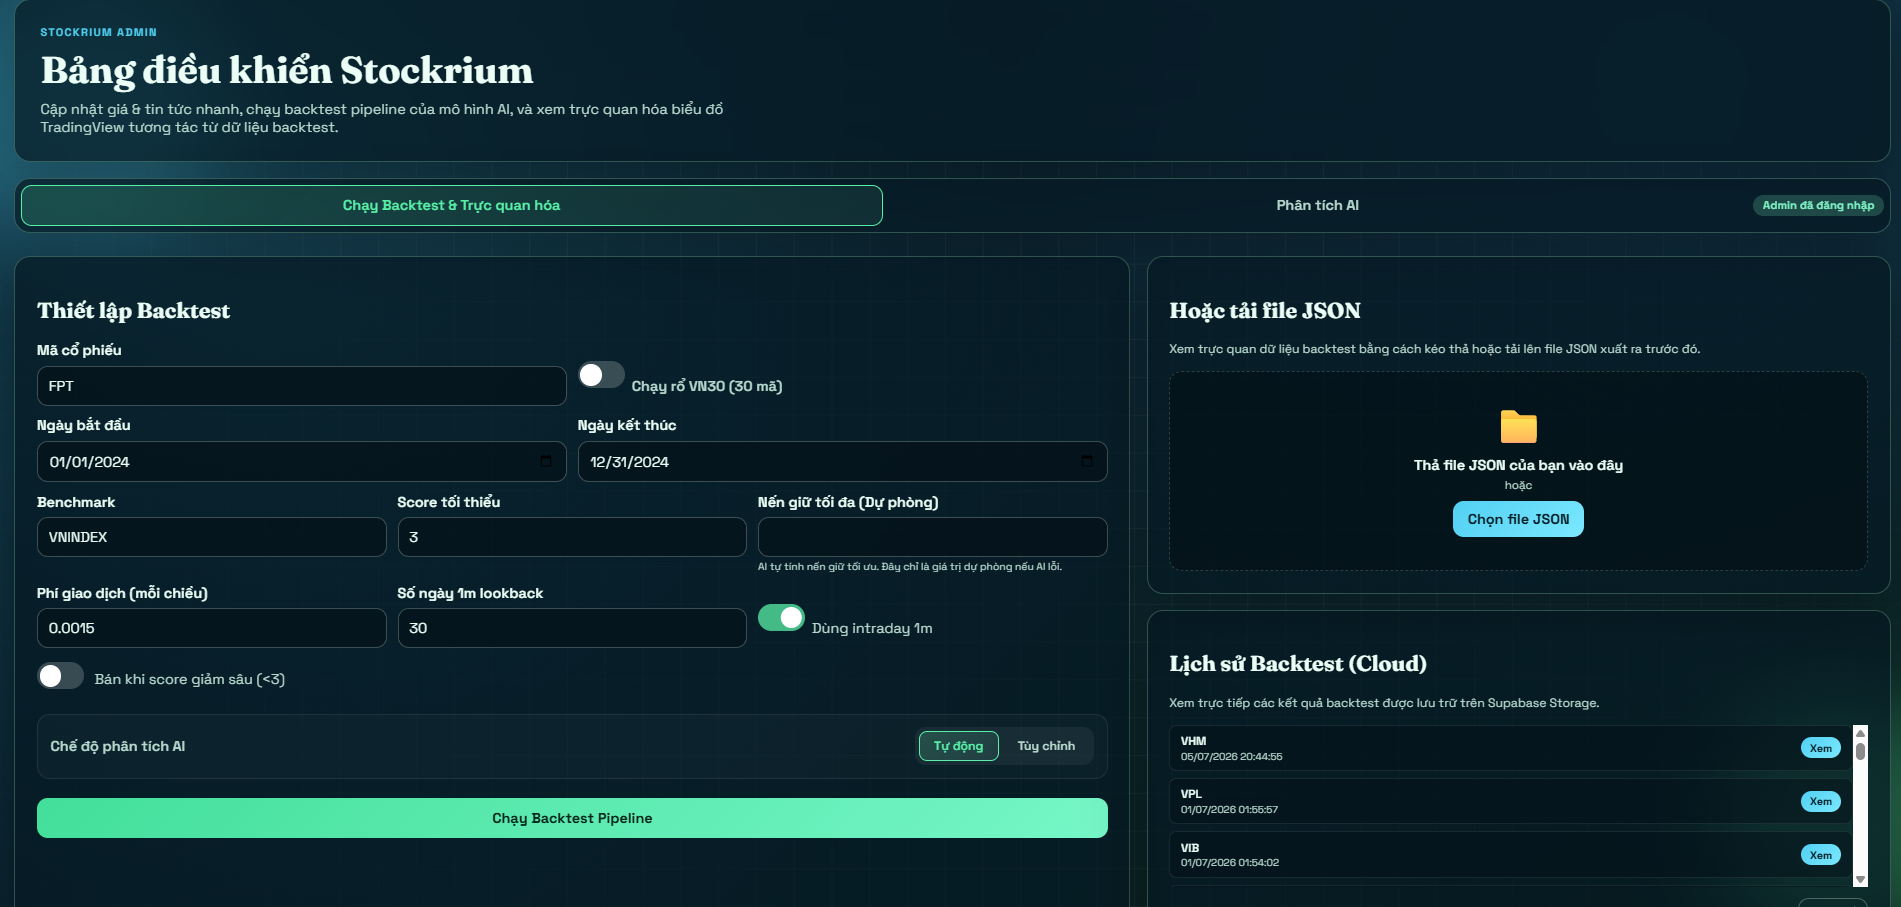
\includegraphics[width=\textwidth,height=0.78\textheight,keepaspectratio]{screenshots/web1.png}
    \caption{Stockrium Lab backtest configuration and saved-run access}
    \label{fig:stockrium-captures8}
\end{figure}

The configuration screen in Figure~\ref{fig:stockrium-captures8} records the security or supported basket, historical period, benchmark, score threshold, transaction fee, lookback window, holding-period fallback, and analysis mode before the user starts a backtest. A submitted backtest becomes a user-owned saved run whose progress is updated asynchronously. Previously saved results or supported JSON artifacts can be reopened for inspection without repeating the computation.

\begin{figure}[H]
    \centering
    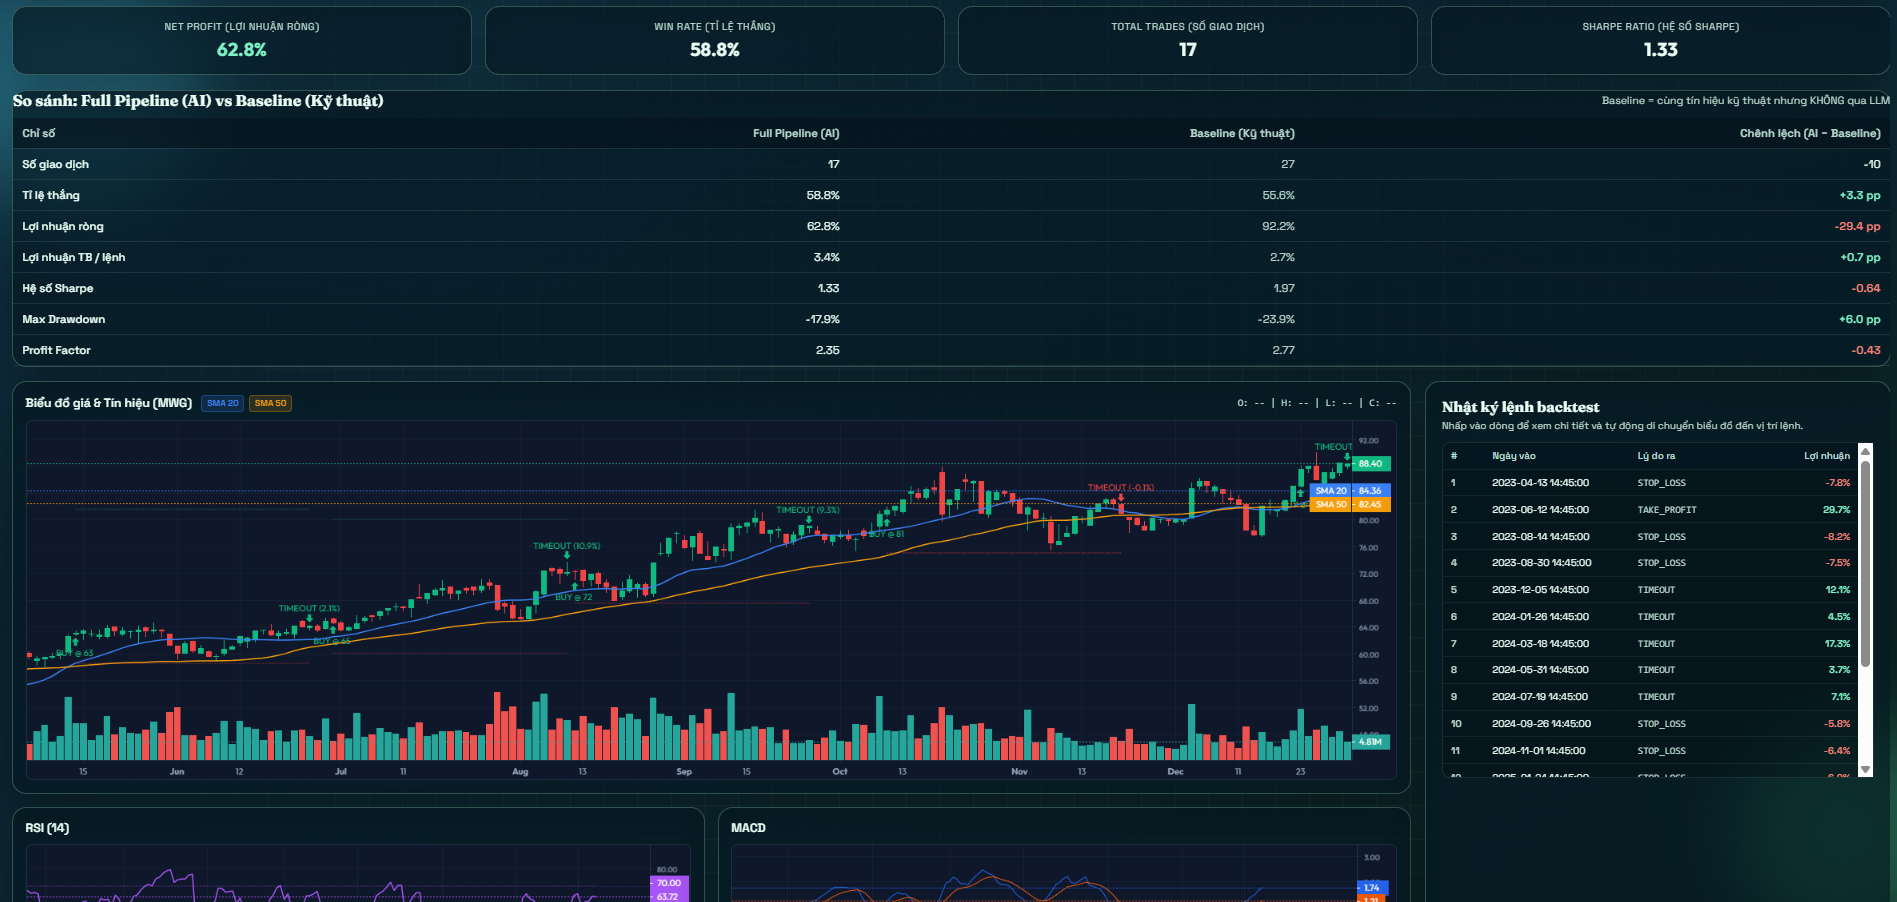
\includegraphics[width=\textwidth,height=0.78\textheight,keepaspectratio]{screenshots/web2.png}
    \caption{Inspection of a Stockrium Lab backtest result}
    \label{fig:stockrium-captures9}
\end{figure}

The result view in Figure~\ref{fig:stockrium-captures9} combines summary metrics with the available full-pipeline and technical-reference outputs. Entry and exit markers on the price chart and the associated trade journal make individual historical outcomes traceable. These values document what the tool produced under the selected configuration; they do not establish future profitability or the superiority of an investment strategy.

\begin{figure}[H]
    \centering
    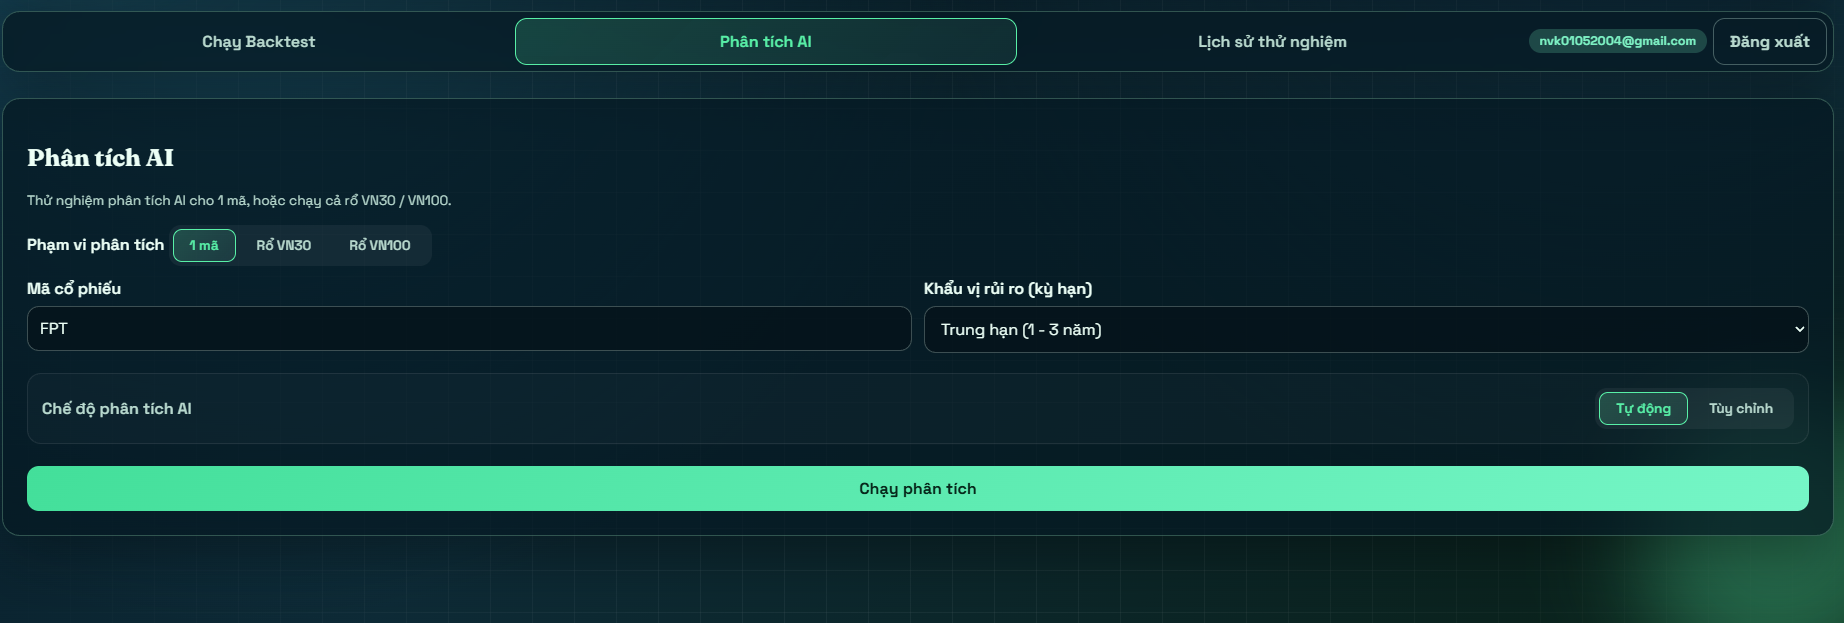
\includegraphics[width=\textwidth,height=0.78\textheight,keepaspectratio]{screenshots/web3.png}
    \caption{Stockrium Lab AI-analysis configuration}
    \label{fig:stockrium-captures10}
\end{figure}

Figure~\ref{fig:stockrium-captures10} allows a user to select one symbol or a supported stock universe, choose automatic or manual evidence settings, and start the multi-agent analysis. For a basket run, the interface can present progress and retain the completed or failed status of the corresponding saved record instead of requiring the initiating web request to remain open.

\begin{figure}[H]
    \centering
    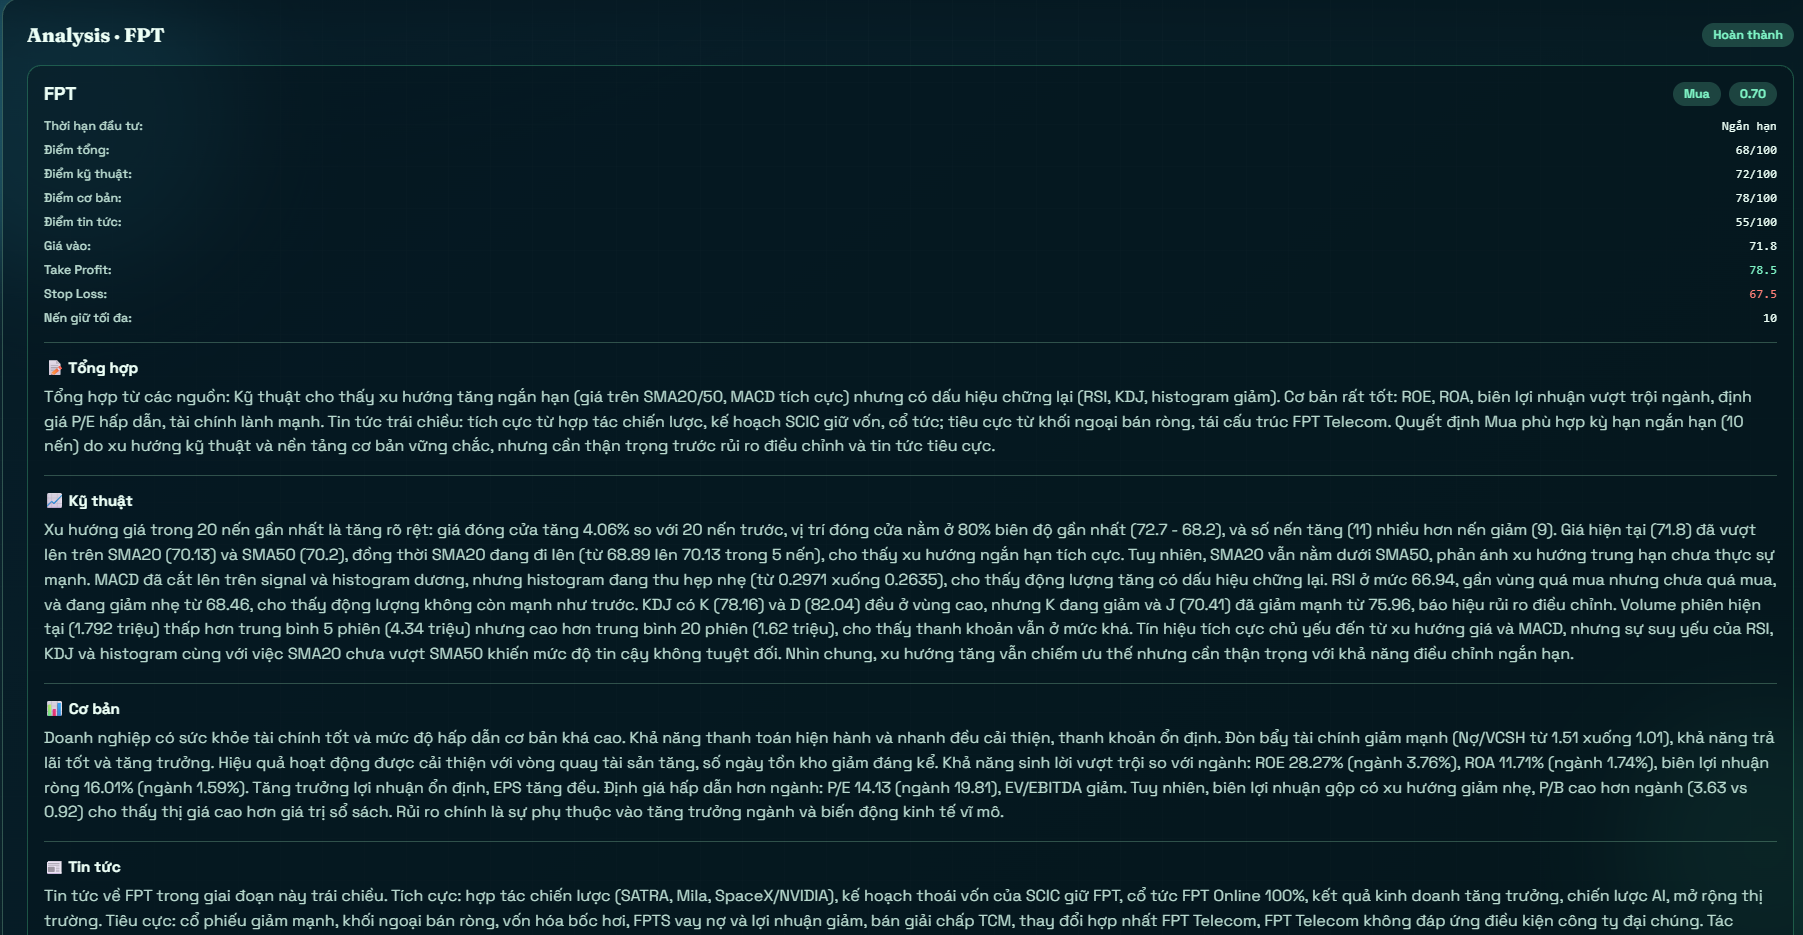
\includegraphics[width=\textwidth,height=0.78\textheight,keepaspectratio]{screenshots/web4.png}
    \caption{Inspection of a Stockrium Lab AI-analysis result}
    \label{fig:stockrium-captures11}
\end{figure}

Figure~\ref{fig:stockrium-captures11} exposes the aggregate assessment together with the technical, fundamental, and news evidence and explanations for the selected symbol. The user can therefore inspect how the multi-agent output was assembled rather than receiving only a final Buy-or-Wait label.

Beyond the detail views shown above, the Stockrium Lab history interface lists the current user's saved runs and supports filtering by run type and status. A user can reopen a completed record or select two to five owned records of the same type for side-by-side comparison of configurations, reproducibility metadata, and supported result fields. Ownership checks apply to history, details, comparisons, and stored artifacts, preventing one account from inspecting another account's results.

Together, the screenshots demonstrate the intended division of work between Stockrium's clients: the mobile application supports frequent, compact investor tasks, whereas Stockrium Lab supports configuration, waiting, saved-result inspection, and comparison on the web. Both interfaces provide decision-support information only and remain separate from real securities order execution.
